\newif\ifcode

\codefalse

\newif\iftwocol
\newif\ifplacefig
\newif\ifdraft
\newif\ifinclfig
\newif\ifieee

% For IEEE 
%\ieeetrue
%\twocoltrue
%\placefigtrue
%\inclfigtrue % false for word count (no figs)
%\draftfalse

% For Draft
\ieeefalse
\twocolfalse
\placefigtrue
\inclfigtrue
\drafttrue

% For ApJ preprint
%\ieeefalse
%\twocolfalse
%\placefigfalse
%\inclfigtrue
%\draftfalse

% For ArXiv
%\ieeefalse
%\twocoltrue
%\placefigtrue
%\inclfigtrue
%\draftfalse

%---------------------------------------------------------------------------------
% PREAMBLE
\iftwocol
	\ifieee
		\documentclass[journal]{IEEEtran}
	\else
		\documentclass[apj]{emulateapj}
	\fi
\else
	\ifieee
		\documentclass[peerreview]{IEEEtran}
	\else
		\documentclass[preprint]{aastex6}
	\fi
\fi

\pdfoutput=1
\usepackage[normalem]{ulem}
\usepackage{color}
\usepackage{graphicx}
\usepackage{enumerate}
\usepackage{listings}
\usepackage{amsmath}
\usepackage{algorithm}
\usepackage{algpseudocode}
%\usepackage[noend]{algpseudocode}
\usepackage{caption}
\algblockdefx[Try]{Try}{EndTry}%
	{\textbf{try}}%
	{\textbf{end try}}
\algcblockdefx[TryExcept]{Try}{Except}{EndTry}%
	{\textbf{except}}%
	{\textbf{end try}}
\algblockdefx[class]{Class}{EndClass}%
	[2]{\textbf{class} {\sc #1}(#2)}%
	{\textbf{end class}}
\algblockdefx[classmethod]{ClassMethod}{EndClassMethod}%
	[2]{\textbf{method} {\sc #1}(#2)}%
	{\textbf{end method}}
\usepackage[toc,page]{appendix}
	
%\DeclareCaptionFormat{algor}{%
%  \hrulefill\par\offinterlineskip\vskip1pt%
%    \textbf{#1#2}#3\offinterlineskip\hrulefill}
%\DeclareCaptionStyle{algori}{singlelinecheck=off,format=algor,labelsep=space}
%\captionsetup[algorithm]{style=algori}
	
	
\ifdraft
	\ifieee
		\usepackage[numbers]{natbib}
		\bibliographystyle{ieeetr}
	\else
		\usepackage{natbib}
		\citestyle{apj}
		\bibliographystyle{apj}
		\bibpunct[,]{(}{)}{;}{a}{}{,}
	\fi
\else
	\ifieee
		\usepackage[numbers]{natbib}
		\bibliographystyle{ieeetr}
	\fi
\fi

\usepackage[bookmarks=false]{hyperref}

\ifieee
\usepackage{etoolbox}
\makeatletter
\patchcmd{\@makecaption}
  {\scshape}
  {}
  {}
  {}
\makeatletter
\patchcmd{\@makecaption}
  {\\}
  {.\ }
  {}
  {}
\def\tablename{Table}
\makeatother
\else
%\makeatletter
\fi

%---------------------------------------------------------------------------------
% CONTROL THINGS
\newcommand{\todo}[1]{{\color{red}{#1}}}
\newcommand{\addref}{{\color{red}(ref. needed)}}
\newcommand{\Msol}{\,M$_{\odot}$}
\newcommand{\TB}{\,Tbytes}
\newcommand{\pippkg}{{\tt yggdrasil-framework}}
\newcommand{\condapkg}{{\tt yggdrasil}}
\newcommand{\pkg}{{\tt yggdrasil}{}}
\newcommand{\cis}{{\tt cis\_interface}{}}
\newcommand{\pkglink}{yggdrasil}
%\newcommand{\pkg}{{\tt \todo{cis\_interface}}{}}
\newcommand{\pkgrun}{{\tt yggrun}}
\newcommand{\A}{Appendix{ }}
\newcommand{\hrefgit}[1]{\href{https://github.com/cropsinsilico/yggdrasil}{{#1}}}
\newcommand{\hrefdoc}[1]{\href{https://cropsinsilico.github.io/yggdrasil/}{{#1}}}
\newcommand{\hrefhack}[1]{\href{https://cropsinsilico.github.io/yggdrasil/hackathon2018/index.html}{{#1}}}

%---------------------------------------------------------------------------------
% SOURCE CODE
\newcommand{\rootsrc}{\lstinputlisting[language=C,label={lst:src:root},caption={root.h: Source code for root model in C.}]{../../yggdrasil/examples/root_to_shoot/src/root.h}}
\newcommand{\shootsrc}{\lstinputlisting[language=Python,label={lst:src:shoot},caption={shoot.py: Source code for shoot model in Python.}]{../../yggdrasil/examples/root_to_shoot/src/shoot.py}}

%---------------------------------------------------------------------------------
% WRAPPER CODE
\newcommand{\rootwrap}{\lstinputlisting[language=C,label={lst:wrap:root},caption={root\_wrapper.c: Wrapper source code for root model in C.}]{../../yggdrasil/examples/root_to_shoot/src/root_wrapper.c}}
\newcommand{\shootwrap}{\lstinputlisting[language=Python,label={lst:wrap:shoot},caption={shoot\_wrapper.py: Wrapper source code for shoot model in Python}]{../../yggdrasil/examples/root_to_shoot/src/shoot_wrapper.py}}

%---------------------------------------------------------------------------------
% YAML FILES
\newcommand{\rootyml}{\lstinputlisting[label={lst:yml:root},caption={root.yml: Model YAML specification file for root model.}]{../../yggdrasil/examples/root_to_shoot/root.yml}}
\newcommand{\shootyml}{\lstinputlisting[label={lst:yml:shoot},caption={shoot.yml: Model YAML specification file for shoot model.}]{../../yggdrasil/examples/root_to_shoot/shoot.yml}}
\newcommand{\rootymlfiles}{\lstinputlisting[label={lst:yml:root_files},caption={root\_files.yml: Connection YAML specification file for running the root model in isolation.}]{../../yggdrasil/examples/root_to_shoot/root_files.yml}}
\newcommand{\shootymlfiles}{\lstinputlisting[label={lst:yml:shoot_files},caption={shoot\_files.yml: Model YAML specification file for running the shoot model in isolation.}]{../../yggdrasil/examples/root_to_shoot/shoot_files.yml}}
\newcommand{\intyml}{\lstinputlisting[label={lst:yml:int},caption={root\_to\_shoot.yml: Connection YAML specification file for the root/shoot integration.}]{../../yggdrasil/examples/root_to_shoot/root_to_shoot.yml}}

%---------------------------------------------------------------------------------
% CODE STYLE
\usepackage{color}
 
\definecolor{codegreen}{rgb}{0,0.6,0}
\definecolor{codegray}{rgb}{0.5,0.5,0.5}
\definecolor{codepurple}{rgb}{0.58,0,0.82}
\definecolor{backcolour}{rgb}{1,1,1}
%\definecolor{backcolour}{rgb}{0.95,0.95,0.92}

\lstdefinestyle{mystyle}{
    backgroundcolor=\color{backcolour},   
    commentstyle=\color{codegreen},
    keywordstyle=\color{magenta},
    numberstyle=\tiny\color{codegray},
    stringstyle=\color{codepurple},
    basicstyle=\footnotesize,
    breakatwhitespace=false,         
    breaklines=true,                 
    captionpos=b,                    
    keepspaces=true,                 
    numbers=left,                    
    numbersep=5pt,                  
    showspaces=false,                
    showstringspaces=false,
    showtabs=false,                  
    tabsize=2
}

\lstset{style=mystyle}


%---------------------------------------------------------------------------------
% MANUSCRIPT INFO
\begin{document}

\ifieee
\else
	\shorttitle{{\pkg}}
\fi

\title{{\pkg}: A Python Package for Integrating Computational Models Across Languages and Scales}

\ifieee
	\author{Meagan~Lang%
	\thanks{The authors are with the National Center for Supercomputing Application, University of Illinois, Urbana-Champaign, IL 61801 USA (e-mail: langmm@illinois.edu)}}
\else
	\author{Meagan~Lang\altaffilmark{1}}

	\altaffiltext{1}{National Center for Supercomputing Application, University of Illinois, Urbana-Champaign, IL email: {\tt langmm@illinois.edu}}
\fi


\ifieee
	\maketitle
\fi

%---------------------------------------------------------------------------------
% ABSTRACT (145 words)
\begin{abstract}
Thousands of computational models have been created within both the plant biology community and broader scientific communities in the past two decades that have the potential to be combined into complex integration networks capable of capturing more complex biological processes than possible with isolated models. However, the technological barriers introduced by differences in language and data formats has slowed this progress. We present \hrefgit{\pkg} (previously {\cis}), a Python package for running integration networks with connections between models across languages and scales. {\pkg} coordinates parallel execution of models in Python, C, C++, and Matlab on Linux, Mac OS, and Windows operating systems, and handles communication in a number of data formats common to computational plant modeling. {\pkg} is designed to be user-friendly and can be accessed at {\tt https://github.com/cropsinsilico/\pkglink}. Although originally developed for plant models, {\pkg} can be used to connect computational models from any domain.
\end{abstract}

\ifieee
	\begin{IEEEkeywords}
		Plant Modeling, Modeling, Communication, Computational Framework, Model Integration, Parallel Processing
	\end{IEEEkeywords}
	\IEEEpeerreviewmaketitle
\else
	\maketitle
\fi

%---------------------------------------------------------------------------------
%---------------------------------------------------------------------------------
% INTRO (183 words)
\section{Introduction}\label{S:intro}
%
%\IEEEPARstart{C}{omputational} 
Plant biologists have produced a wealth of computational models to describe the biological processes governing plant growth and development, covering scales from atomistic to global. Although usually developed independently to address questions specific to an organ, species, or growth process, computational plant models can also have applications beyond their original scope. Many biological processes are the same across different species of plants, allowing models developed for one species to be adapted for another by modifying input parameters. In addition, computational models for different scales, organs, or processes are often related via biological dependencies. %can also be combined, or integrated, to probe more complex biological mechanisms. 
%By integrating a metabolic flux model with a genetic regulatory model for carbon uptake, 
%%
%\ifieee
%	\citep{integration_prep} 
%\else
%	\citet{integration_prep} 
%\fi
%%
%was able to identify gene candidates for regulating photosynthesis under elevated CO$_{2}$. 
With advances in computational power, it should be possible to link biologically-related models to create complex integration networks capable of capturing the response of entire plants, fields, or regions. However, independently developed computational models often have compatibility issues resulting from differences in programming language or data format that make such collaborations difficult. 

Consider the task of integrating a simple root growth model with a shoot growth model. Our example root growth model is written in C (see Listing \ref{lst:src:root}) and can be expressed as
\begin{equation}
R_{t+1} = R_{t} \times r_{r} \times dt + R_{t}.
\end{equation}
The inputs to the root growth model are
\begin{itemize}
	\item $R_{t}$: the root mass at time $t$ (g)
	\item $r_{r}$: the relative root growth rate (hr$^{-1}$)
	\item $dt$: the time step (hr)
\end{itemize}
and the output of the root growth model is $R_{t+1}$, the root mass at the next time step. 
%
The shoot growth model is written in Python (see Listing \ref{lst:src:shoot}) and can be expressed as
\begin{equation}
S_{t+1} = S_{t} \times r_{s} \times dt + S_{t} - (R_{t+1} - R_{t}).
\end{equation}
The inputs to the shoot model are 
\begin{itemize}
	\item $S_{t}$: the shoot mass at time $t$ (kg)
	\item $r_{s}$: the relative shoot growth rate (d$^{-1}$)
	\item $dt$: the time step (d)
	\item $R_{t}$: the root mass at time $t$ (kg)
	\item $R_{t+1}$: the root mass at time $t+1$ (kg)
\end{itemize}
and the output of the shoot growth model is $S_{t+1}$, the shoot mass at the next time step.
%
While it is possible to run both models in isolation if all of the appropriate input variables are provided, the value of $R_{t+1}$ calculated by the root growth model could be used as input to the shoot growth model. However, because the two models are written in different languages, the two models cannot be directly integrated. To integrate the models a scientist must either "manually" integrate them by running one model and then the other or translate one of the models into the language of the other so that it can be called directly. For a tightly coupled set of models such as these where one model depends directly on the result from the other at the current time step, manual integration is very inefficient for more than a handful of time steps even when done using a script. Although translating one or both of these simple toy models would be relatively straight forward, actual plant models are much more complex and could contain thousands of lines of code that would be time consuming to translate and result in unnecessary duplication of model algorithms.

We present an Open Source Python package, {\pkg}, for creating and running integration networks by connecting existing computational models written in different programming languages. {\pkg} was developed as part of the Crops \emph{in Silico} \citep{Marshall-Colon2017} initiative to build a complete crop \emph{in silico} from the level of the genes to the level of the field. {\pkg} is available on Github\footnote{{\tt https://github.com/cropsinsilico/\pkglink}} with full documentation\footnote{{\tt https://cropsinsilico.github.io/\pkglink/}} and can be installed from PyPI\footnote{{\tt https://pypi.org/project/\pkglink/}} via {\tt pip install {\pippkg}} or conda-forge\footnote{{\tt https://github.com/conda-forge/\pkglink-feedstock}} via {\tt conda -c conda-forge install {\condapkg}}. Although developed for the purpose of integrating plant biology models, {\pkg} can be applied to any situation requiring coordination between models in the supported languages. \S\ref{S:background} provides background information on existing efforts for cross-language model integration, \S\ref{S:methods} describes the methods used by the {\pkg} package to integrate models, \S\ref{S:example} provides a worked example of integrating the two model presented above, \S\ref{S:results} presents several tests demonstrating the performance of message passing between integrated models, and \S\ref{S:discuss} describes a few use cases for {\pkg}, 
summarizes the features and limitations of the {\pkg} package, and outlines areas of ongoing and future development.

%---------------------------------------------------------------------------------
%---------------------------------------------------------------------------------
% BACKGROUND
\section{Background}\label{S:background}
%
Computational plant models are usually written with a very specific research question in mind \citep[e.g. describing a specific metabolic pathway in C4 photosynthesis,][]{Wang2014}. The resulting model codes are often highly tuned for this one purpose and are written specifically for scientists within an isolated group of collaborators. As a result, it is unlikely that models produced by two independent groups will be directly compatible in terms of language, data format, or units \citep{Marshall-Colon2017}. 

There are models written in Matlab \citep{ZHU2013, Wang2014}, Python \citep{Pradal2009}, C++ \citep{Merks2011, Postma2017}, Microsoft Excel \citep{Sharkey2016}, VisualBasic \citep{Humphries1995, HALL2013}, R \citep{WANG2015}, Java \citep{Song2013, Kappas2013}, Fortran \citep{Goudriaan1994}, and several domain specific languages \citep[e.g. SBML,][]{Hucka2003}. The variety of data formats used by these codes is just as diverse. While some specific subfields have settled on standards for things like microarray gene expression data \citep[e.g. MINiML,][]{GEO2017}, many models use unique data formats that may or may not include metadata such as the data types, field names, or units. 
%For example, OpenAlea \citep{Pradal2008} defines its own Multiscale Tree Graph (MTG) tree structure for describing plant topology at different scales that is an extension to the MTG format used by AMAPmod \citep{Godin1998}. 
For example, while LPy \citep{Boudon2012} and Houdini FX \citep{HoudiniFX} both allow users to specify plant structures via L-systems, they differ slightly in their syntax and so are not directly compatible. Or, as another example, 3D canopy structures can be generated in any unit and standard 3D geometry formats like Ply \citep{ply} and Obj \citep{obj} do not include units in their metadata. As a result, if an LPy model produces a canopy in Ply format with units of centimeters, the photosynthetic photon flux density (PPFD) output by a ray tracer like fastTracer \citep{Song2013} (which expects a geometry in units of meters) would be incorrect. 

As a result, integrating two biological models like the root and shoot models from \S\ref{S:intro} requires that the following questions be addressed first:
%
\begin{enumerate}
	\item Orchestration: How will models be executed?
	\item Communication: How will information be passed from one model to the next across languages?
	\item Translation: How will data output by one model be translated into a format understood by the next model?
\end{enumerate}

These three questions can be addressed through manual integration (e.g. running the root model, converting the output root mass into the units expected by the shoot model, and then running the shoot model). However, manual integration is 1) computationally inefficient when many iterations are necessary, such as during parameter searches or steady state convergence tests, 2) unique to every integration, requiring the production of new scripts, 3) time consuming, 4) prone to error, and 5) complex when more than three models are being integrated. Within both computational biology and the larger scientific computing community, groups have developed around different solutions to the problem of connecting models. These solutions can generally be grouped into two categories: domain specific languages and frameworks.

%---------------------------------------------------------------------------------
% DOMAIN SPECIFIC LANGUAGE
\subsection{Domain Specific Languages (DSLs)}\label{SS:dsl}
%
One solution is to agree upon a language. The questions of orchestration, communication, and translation become trivial when models are all written in the same language. Beyond selecting a single programming language, many communities have  developed dedicated domain specific languages (DSLs) for model representation. For example, the Systems Biology Markup Language \citep[SBML][]{Hucka2003} is an XML-based format for representing models of biological processes. Scientists can compose their models using SBML markup and then run their model using software designed to parse SBML files. Other DSLs for biological models include LPy \citep{Boudon2012}, CellML \citep{Cuellar2003}, FLAME \citep{Coakley2012}, and BioPAX \citep{Demir2010}. Dedicated model DSLs improve the reusability of models written in the DSL and have the advantage of often implicitly handling data transformation. However, they provide no help for existing models that are not written in the DSL or those that cannot be expressed within the constraints of the DSL. Furthermore, learning a new DSL, in addition to a programming language, can be daunting.

%---------------------------------------------------------------------------------
% FRAMEWORKS
\subsection{Workflow/Data Flow/Framework}\label{SS:framework}
%
Another approach is a workflow/data flow/framework tool for models that are written in the same programming language or can be wrapped using an intermediary \citep[e.g. Cython, ][]{Behnel2011a}. For example, there are many generic tools in Python for coordinating the execution of tasks in parallel or serial \citep[e.g.][]{babuji18, celery, luigi}. While these tools are powerful for organizing complex work flows, it is the user's onus to make sure that the components they connect are compatible and handle any data transformation that might be necessary, e.g. unit conversion or field selection.

There are also domain specific frameworks for connecting biological models. For example, OpenAlea \citep{Pradal2015} allows users to compose networks from different components including plant models, analysis tools, and visualization tools. Domain specific frameworks are more intuitive and ultimately more flexible than DSLs in the types of operations they allow models to perform since they have access to the full power of a programming language. However, they are stricter in several respects: 1) the model must be written in (or exposable to), the language of the framework and 2) the model must be written in a way that is aware of the framework and/or the format of models with which it will interact. Like DSLs, frameworks also often provided limited support for models written without the framework in mind. 

{\pkg} is an example of a framework that overcomes these issues by exposing simple and easily accessible interfaces in the languages of the models (See \S\ref{SSS:interface}) that permit messages to be passed between the model processes as they run in parallel (See \S\ref{SS:communication}). As a result, models writers only need knowledge of the language in which their model is written.

%---------------------------------------------------------------------------------
% MESSAGE PASSING TOOLS
%\subsection{Message Passing Tools}\label{SS:messages}
%
%There are many existing software solutions for passing messages between processes. Implementations of the Message Passing Interface (MPI) standard, such as MPICH \citep{Gropp1996} and OpenMPI \citep{Gabriel2004}, allow communication between instances of a program launched on parallel processes with distributed memory. MPI implementations are robust, fast, and scale well, however, they are optimized for processing high volumes of structured data on supercomputers and are not as well suited to the case of dynamic integration networks composed of diverse processes operating on different timescales.

%---------------------------------------------------------------------------------
%---------------------------------------------------------------------------------
% METHODS
\section{Methods}\label{S:methods}

{\pkg} was designed to transform models into building blocks that can be easily combined with other blocks to build complex structures, thus promoting model reuse and collaboration between scientists with varying degrees of overlapping expertise. {\pkg} does so by addressing the questions from \S\ref{S:background} while being:

\begin{itemize}
	\item {\bf Easy to use.} Require as little modification to the model source code as possible and only in the language of the model itself.
	\item {\bf Efficient.} Allow models to run in parallel with asynchronous communication that doesn't block model execution when a message is sent, but has yet to be received.
	\item {\bf Flexible.} Provide the same interface to the user, regardless of the communication mechanism being used or the platform the model is being executed on.
\end{itemize}

{\pkg} is built upon several well-established open-source software packages (see below) along with new tools developed explicitly for {\pkg} including utilities for running and monitoring models written in other languages from Python, dynamically creating and managing communication networks, data type conversions between languages, and asynchronous message passing with variable underlying communication mechanisms. {\pkg} currently support models written in Python, Matlab, C, and C++ with additional Domain Specific Language (DSL) support for LPy models \citep{Boudon2012}. Support for additional languages is planned for future development (See \S\ref{SS:langsupport}).

%---------------------------------------------------------------------------------
% ORCHESTRATION
\subsection{Orchestration}\label{SS:orchestration}
%
{\pkg} is executed via a command line interface (CLI), {\pkgrun} with specification files (\S\ref{SSS:yaml}) as input. Based on the information contained in the specification files, {\pkg} dynamically establishes a network of asynchronous communication channels (\S\ref{SS:communication}), and launches the models on new processes (\S\ref{SS:model_execution}). Although written in Python, {\pkg} was written such that users need not have any knowledge of the Python language and can interact with {\pkg} solely through the CLI. In addition to the CLI, more advanced capabilities are also exposed via the Python API including access to more detailed information about the running integration.
%At execution, {\pkg} launches models on new processes based on information contained in a YAML specification file (See \S\ref{SSS:yaml} below) and establishes 

%---------------------------------------------------------------------------------
% YAML
\subsubsection{Specification Files}\label{SSS:yaml}
%
Users specify information about models and integration networks via declarative YAML files \citep{Ben-Kiki2009}. The YAML file format was selected because it is human readable and there are many existing tools for parsing YAML formats in different programming languages \citep[e.g.][]{Simonov2006,pyyaml,jsyaml}. The declarative format allows user to specify exactly what they want to do, without describing how it should be done. While the information about models and integration networks can be contained in a single YAML file, the information can naturally be split between two or more files, one (or more) containing information about the model(s) and one containing the connections comprising the integration network. This separation is advantageous because the model YAML can be re-used, unchanged, in conjunction with other integration networks. 

Model YAMLs include information about the location of the model source code, the language the model is written in, how the model should be run, and any input or output variables including their data type (e.g. array, scalar, mesh) and physical units. 
%
%For example, Listings \ref{lst:yml:root} and \ref{lst:yml:shoot} from \A\ref{A:yml} are the model YAMLs for the example root and shoot growth models from \S\ref{S:intro}. These model YAMLs could be used in any integration without being modified because the model inputs and outputs will not change.
%
%\rootyml
%
%\shootyml
%
Integration networks are specified by declaring the connections between models and connections are declared by pairing an output variable from one model with the input variable of another model. The {\pkg} CLI sets up the necessary communication mechanisms to then direct data from one model to the next in the specified pattern. Models can have as many input and/or output variables as is desired and connections between models are specified by references to the input/output variables associated with each model. In addition, input and output variables can also be connected to files.
%
%For example, in the connection YAML for integrating the root and shoot models (Listing \ref{lst:yml:int} from \A\ref{A:yml}), the first two connections link the {\tt root\_input} and {\tt shoot\_input} input channels from the root and shoot model YAML's to input files. The third connection links the {\tt next\_root\_mass} output variable from the root model YAML (Listing \ref{lst:yml:root}) to the {\tt next\_root\_mass} input variable from the shoot model YAML (Listing \ref{lst:yml:shoot}). The forth connection links the {\tt next\_shoot\_mass} to an output file.
%
%\intyml
%
This format allows users the flexibility to create complex integration networks and test models in isolation before running the entire integration network as will be seen in \S\ref{S:example}.


%---------------------------------------------------------------------------------
% MODEL EXECUTION
\subsubsection{Model Execution}\label{SS:model_execution}
%
{\pkg} launches each model in an integration in its own process, allowing models to complete independent operations in parallel and complete tasks more quickly. For example, the root and shoot growth models from \S\ref{S:intro} (described further in \S\ref{S:example}) require 10.28\,s and 10.40\,s respectively to run for 100 time steps in isolation with direct input/output from/to files in their native language. If these two models were manually integrated in serial via the command line, the integration would require a total of 20.68\,s. However, because {\pkg} offers parallel execution of the models, the same integration requires only 16.03\,s when using {\pkg}, a speed-up of 1.29. The exact speedup provided by parallel integration using {\pkg} depends on how independent the models are and how equally distributed the work is between the models. If the models are fully independent, the speedup is limited by the time required to execute the slowest model. If the models are dependent on one-another, the models may have to wait to receive messages and the speedup will not be as great. \S\ref{SS:speedup} provides additional information about the speedups achievable through {\pkg} parallel integration and how model structure influences the size of the performance boost.

While every model is executed in a new process, how the model is handled depends on the language it is written in. {\pkg} has a dedicated driver for each of the supported languages with utilities that allow {\pkg} to launch and monitor executables written in that language from Python. Models written in interpreted languages (Python and Matlab) are executed on the command line via the interpreter. In the case of Matlab, where a significant amount of time is required to start the Matlab interpreter (see \S\ref{SS:results_language}), Matlab shared engines are used to execute Matlab models. Matlab shared engines are Matlab instances that other processes can submit Matlab code to for execution. While shared engines also require the same amount of time to start as a standard instance of the Matlab interpreter, they can be started in advance and then reused.

For the compiled languages (C and C++) there are a few options. The user can compile the model themselves, provided they include the source code for the appropriate dependencies at compilation and link against the appropriate {\pkg} header library. {\pkg} provides several command line tools for determining the locations of the necessary libraries and any required compilation/linking flags. Alternatively, users can provide the location of the model source code and let one of several {\pkg} drivers handle the compilation, including linking against the appropriate {\pkg} interface library. {\pkg} also has support for compiling models using Make \citep{Stallman2004} and CMake \citep{Martin2006} for models that already have a Makefile or CMakeLists.txt. To use these tools to compile a model, lines are added to the recipe in order to allow linking against {\pkg}.

Once the models are running, {\pkg} uses threads on the master process to monitor the progress of the model and report back model output (e.g. log messages printed to stdout or stderr) and any status changes. If a model issues any errors, the master process will shut down any model processes that are still running and close any connections, discarding any unprocessed messages. If a model completes without any errors, the master process will cleanup any connections that are no longer required after waiting for all messages to be processed. The master process will only complete once an error is encountered or all model processes have completed.

The algorithms for a generic model driver and the master thread are provided as Algorithms \ref{alg:model} \& \ref{alg:master} respectively in \A\ref{A:algorithms}.

%---------------------------------------------------------------------------------
% COMMUNICATION
\subsection{Communication}\label{SS:communication}
%
Integrating models requires that they are able to send and receive information to and from other models written in different languages via some communication mechanism. Communication within {\pkg} integration networks was designed to be flexible in terms of the languages, platforms, and data types available. To accomplish this, {\pkg} leverages three different tools for communication, System V IPC Queues (\S\ref{SSS:ipc}), ZeroMQ (\S\ref{SSS:zmq}), and RabbitMQ (\S\ref{SSS:rmq}), which each have their own strengths and weaknesses. The particular communication mechanism used by {\pkg} is determined by the platform, available libraries, and integration strategy. However, regardless of the communication mechanisms, the user will always use the same interface in the language of their model, simplifying the number of routines that users need to use for integration (see \S\ref{SSS:interface}).

{\pkg} includes its own implementation of asynchronous communication via each of the communication mechanisms that are supported. While there are existing tools for asynchronous communication using each of these communication mechanisms, using a tool developed specifically for {\pkg} allows for a more uniform treatment of the different communication mechanisms, greater control over how threads are managed (e.g. killing a thread when messages cannot be interpreted), and a more seamless coordination with other {\pkg} processes (e.g. enforcing dependencies on other model and connection threads).

%---------------------------------------------------------------------------------
% SYSTEM V IPC
\subsubsection{System V IPC Queues}\label{SSS:ipc}
%
The first communication mechanism used by {\pkg} was System V interprocess communication (IPC) message queues \citep{Rusling1999} on Posix (Linux and Mac OS X) systems. IPC message queues allow messages to be passed between models running on separate processes on the same machine. While IPC message queues are simple, fast (See \S\ref{SS:results_commtype}), and are built into most Posix operating systems, they do not work in all situations. IPC queues are not natively supported by Windows operating systems and do not allow communication between remote processes. In addition, IPC queues also have relatively low default message size limits on Mac OS X systems (2048 bytes or 256 64 bit numbers). Once the queue is full or if the message is larger than the limit, any process attempting to send an additional message will stop until a sufficient number of messages has been removed from the queue to accommodate the new message. For messages larger than the limit, the sending process will stop indefinitely. This can be handled by splitting large messages into multiple smaller messages (see \S\ref{SSS:large}); however, the time required to send a message increases with the number of message it must be broken into (See \S\ref{SS:results_commtype}). These limits make sending large messages relatively inefficient when compared with other communications mechanisms. As a result, IPC queues are used by {\pkg} only as a fallback on Posix systems if none of the other supported communication libraries have not been installed.

%---------------------------------------------------------------------------------
% ZEROMQ
\subsubsection{ZeroMQ}\label{SSS:zmq}
%
The preferred communication mechanism used by {\pkg} are ZeroMQ sockets \citep[ZMQ][]{Akgul2013}. ZMQ provides broker-less communication via a number of protocols and patterns with bindings in a wide variety of languages that can be installed on Posix and Windows operating systems. ZMQ was adopted by {\pkg} in order to allow support on Windows and for future target languages (See \S\ref{SS:future}) that could not be accomplished using IPC queues. In addition, while ZMQ allows interprocess communication via IPC, ZMQ also supports protocols for distributed communication via an Internet Protocol (IP) network. While {\pkg} does not currently support using these protocols for distributed integration networks, this is an avenue of future development that has been prepared for.

In addition to using the default ZMQ libraries, {\pkg} also includes supporting routines for allowing received messages to be confirmed. Because ZMQ is broker-less, a socket has no way of knowing if the message it sent was successfully received. This lack of confirmation makes it harder to determine if there is was error somewhere along the network. {\pkg} overcomes this by generating two ZMQ sockets for every connection: one for passing the messages and one for confirming them. Each time a message is received, the receiving socket confirmation thread will send a confirmation including a unique ID for the received message and then wait for a reply to that confirmation. The sending socket confirmation thread will continuously check the confirmation sockets for messages indicating that sent messages were received. Once a confirmation message is received, it will send a reply to the receiving confirmation socket and record the ID of the message that was confirmed. This handshake operation ensures that all messages are accounted for so {\pkg} knows if a message is lost and where it was lost.


%---------------------------------------------------------------------------------
% RABBITMQ
\subsubsection{RabbitMQ}\label{SSS:rmq}
%
While broker-less communication like ZMQ is light weight and fast, it is not as fault tolerant as brokered messaging systems that confirm message delivery and can resend dropped messages. Resilience to dropped messages, while not as necessary for integrations running entirely on a local machine, will be more important for integrations running on distributed resources with less reliable connections. As a result, {\pkg} includes support for brokered communication via RabbitMQ \citep[RMQ][]{RMQ} that will be used during future development to allow integrations to run on distributed resources or include remote models run as services (\S\ref{SS:distributed}). Due to the slower message speed, {\pkg} does not currently use RMQ for communication unless explicitly specified by the user in their integration network YAML. 

%---------------------------------------------------------------------------------
% ASYNCHRONOUS MESSAGE MASSING
\subsubsection{Asynchronous Message Passing}\label{SSS:async}
%
The same asynchronous communication strategy is used with each of the communication mechanisms supported by {\pkg}. Models do not block on sending messages to output channels; the model is free to continue working on its task while an \emph{output driver} waits for the message to be routed and received on a separate master process thread. Similarly, an \emph{input driver} continuously checks input channels on another thread, moving received messages into a intermediate buffer queue so that they are ready and waiting for the receiving model when it asks for input. These drivers work together to move message along from one model to the next like a conveyor belt. As a result, models in complex integration networks are not affected by the rate at which dependent model consume their output and the speedup offered by running the models in parallel is improved. Figure \ref{fig:async} describes the general flow of messages, Algorithms \ref{alg:async_send} \& \ref{alg:async_recv} in \A\ref{A:algorithms} describe the asynchronous output \& input channel procedures, and Algorithm \ref{alg:conn} describes the procedure followed by input \& output connection drivers.
%
\ifinclfig
 	\begin{figure}[htbp]
	\begin{center}
	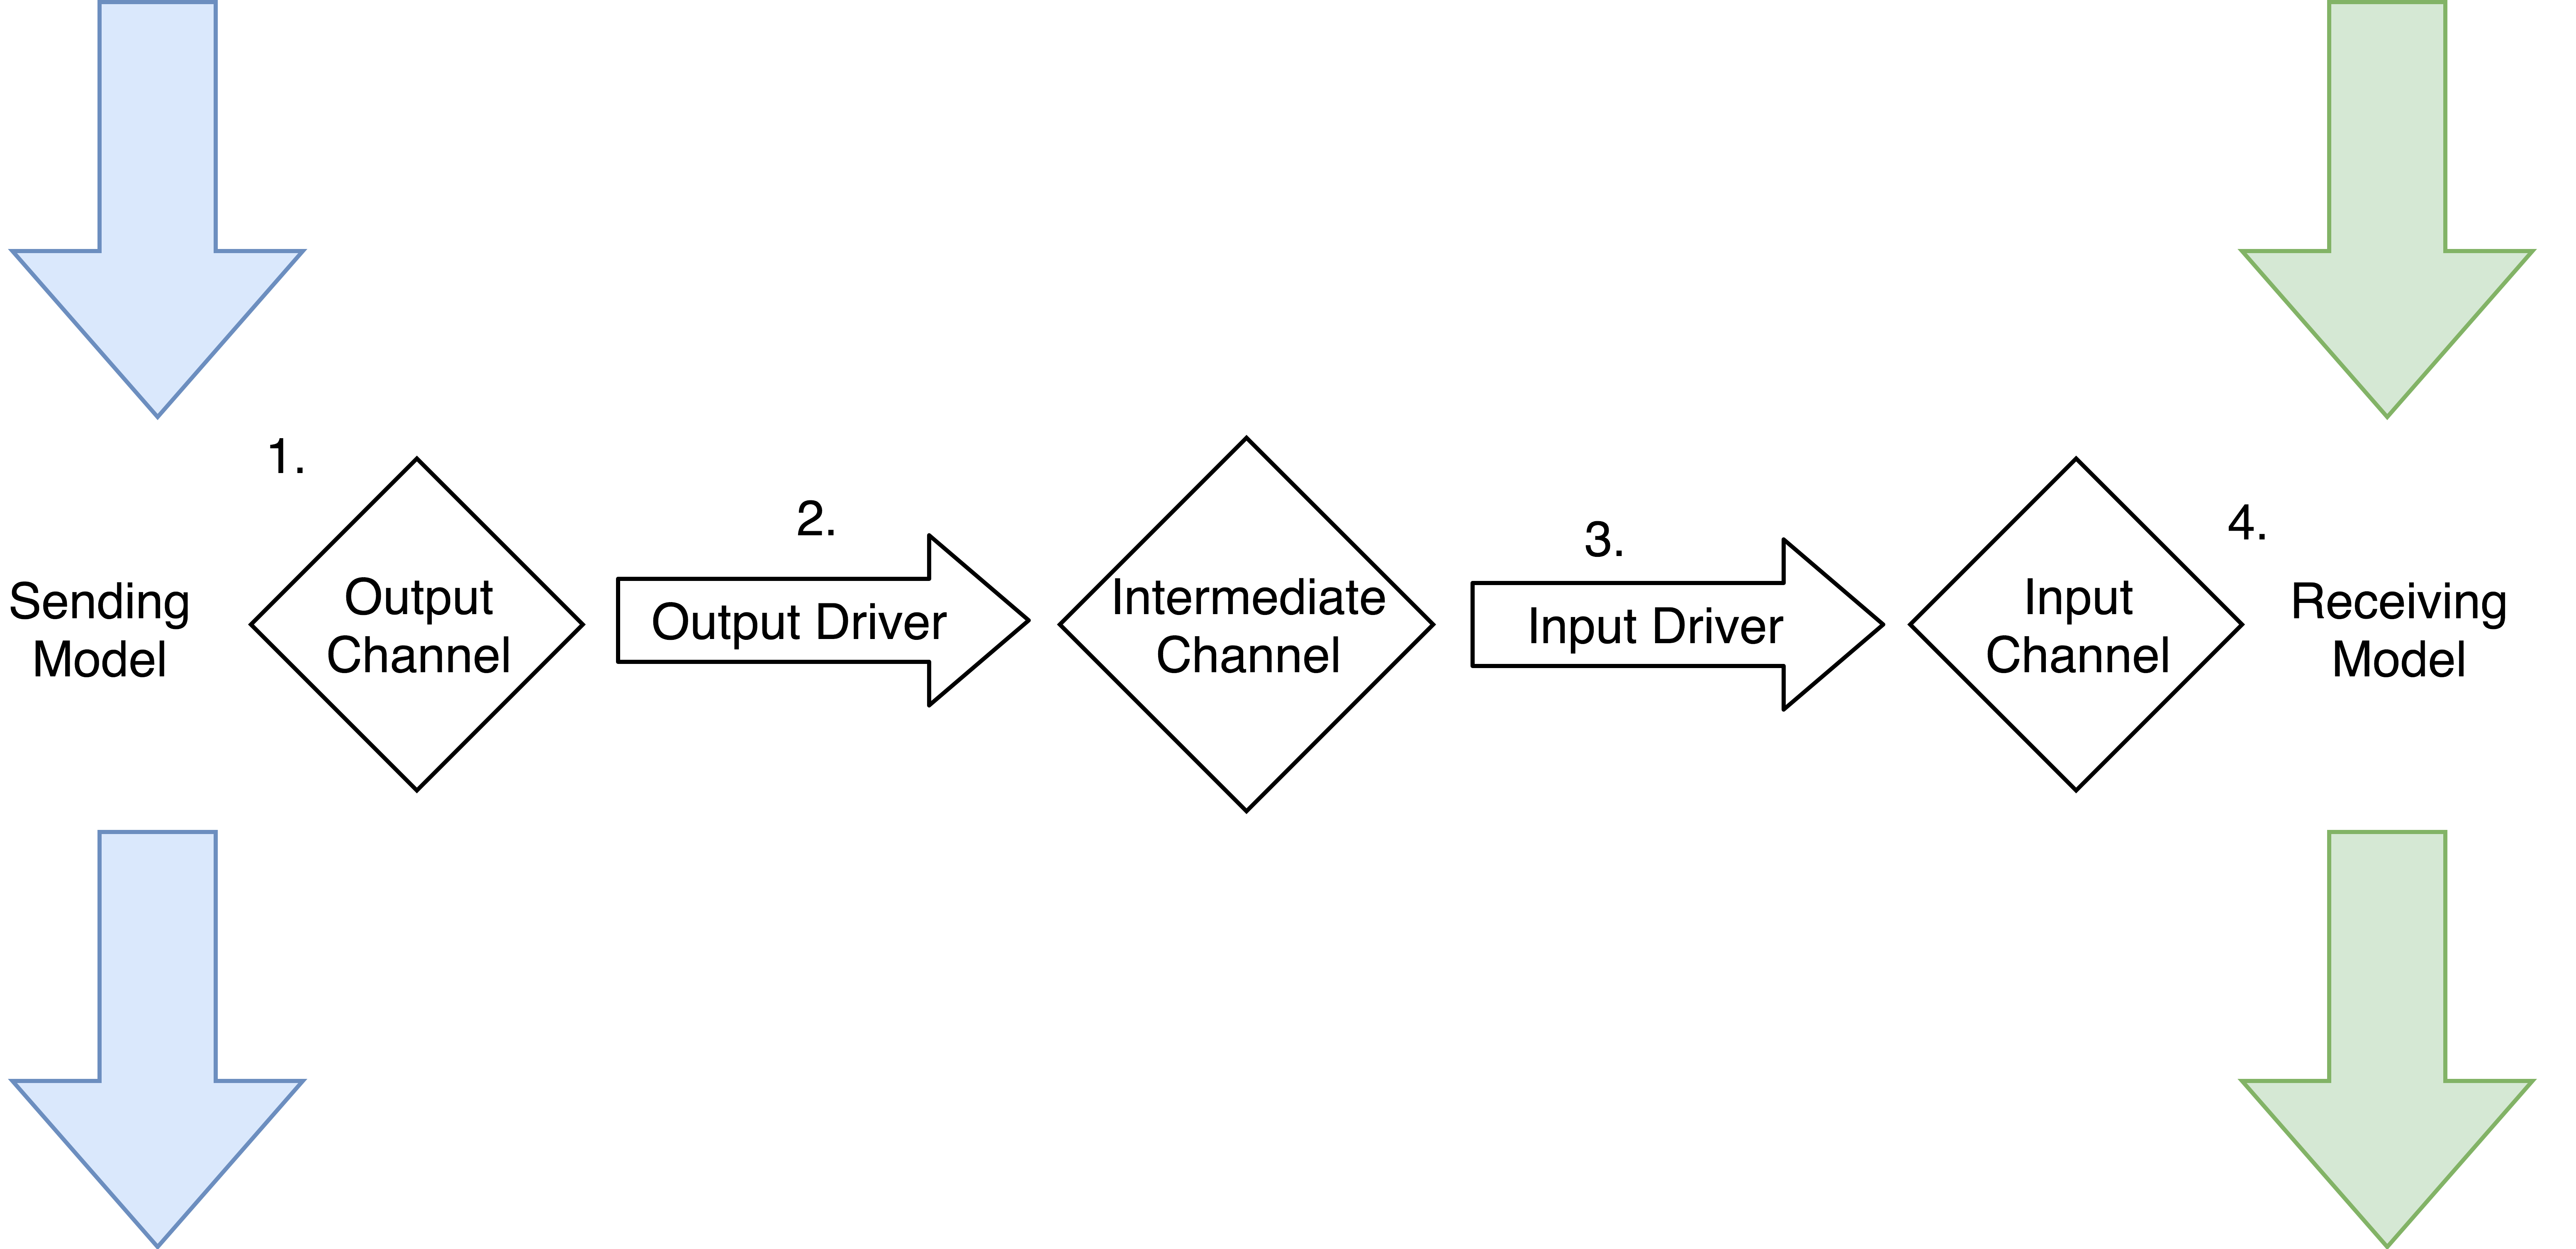
\includegraphics[width=\columnwidth,keepaspectratio]{./images/io_drivers.png}
	\caption{Diagram of how messages are passed asynchronously using input/output drivers and an intermediate channel.}
	\label{fig:async}
	\end{center}
	\end{figure}
\fi
%
\begin{enumerate}
	\item A model sends a message in the form of a native data object via a language-specific API to one of the output channels declared in the model YAML. The output channel interface encodes the message and sends it.
	\item An output connection driver (written in Python) runs in a separate thread on the master process, listening to the model output channel. When the model sends a message, the output connection driver checks that the message is in the expected format and then forwards it to an intermediate channel. The intermediate channel is used as a buffer for support on distributed architectures (e.g. if one model is running on a remote machine). In these cases, the intermediate channel will connect to a RMQ broker using security credentials.
	\item An input connection driver (also written in Python) runs in a separate thread, listening to the intermediate channel. When a message is received, it is then forwarded to the input channel of the receiving model as specified in the integration network YAML.
	\item The receiving model receives the message in the form of an analogous native data object. Interface receive calls can be either blocking or non-blocking, but are blocking by default.
\end{enumerate}


%In addition to communication between two models, users can also specify that a 
%model should receive/send input/output from/to a file. This is specified in 
%the integration network YAML and does not impact the way the model will 
%receive/send messages. In this way, users can test their model integration in 
%isolation with input/output form/to files rather than another model.

%---------------------------------------------------------------------------------
% SENDING/RECEIVING LARGE MESSAGES
\subsubsection{Sending/Receiving Large Messages}\label{SSS:large}
%
All of the communication tools leveraged by {\pkg} have intrinsic limits on the allowed size for a single message. Some of these limits can be quite large ($2^{20}$ bytes for ZMQ and RMQ), while others are very limiting (2048 bytes on Mac OS X for IPC queues). Although messages consisting of a few scalars are unlikely to exceed these limits, biological inputs and outputs are often much more complex. For example, structural data represented as a 3D mesh can easily exceed these limits. To handle messages that are larger than the limit of the communication mechanism being used, {\pkg} splits the message up into multiple smaller messages. In addition, for large messages, {\pkg} creates new, temporary communication channels that are used exclusively for a single message and then destroyed. The address associated with the temporary channel is sent in header information as a message on the main channel along with metadata about the message that will be sent through the temporary channel like size and data type. Temporary channels are used for large messages to prevent mistakenly combining the pieces from two different large messages that were received at the same time such as in the case that a model is receiving input from two different models working in parallel. The procedures for creating and using temporary channels for sending large messages can be seen in the {\sc Send} and {\sc Recv} methods from Algorithms \ref{alg:async_send} \& \ref{alg:async_recv} respectively in \A\ref{A:algorithms}.


%---------------------------------------------------------------------------------
% INTERFACE
\subsubsection{Interface}\label{SSS:interface}
%
{\pkg} provides interface functions/classes for communication that are written in each of the supported languages. Language specific interfaces allow users to program in the language(s) with which they are already familiar.  Each language interface is an implementation of Algorithms \ref{alg:async_send} \& \ref{alg:async_recv} from \A\ref{A:algorithms} that provides users with send and receive calls for passing messages. The Python interface provides communication classes for sending and receiving messages. The Matlab interface provides a simple wrapper class for the Python class, that exposes the appropriate methods and handles conversion between Python and Matlab data types. The C interface provides structures and functions for accessing communication channels and sending/receiving messages. The C++ interface provides classes that wrap the C structures with functions called as methods.

In addition to basic input and output, each interface also provides access to more complex data types and communication patterns that can be found in the {\pkg} documentation. 
%Pseudocode describing the asynchronous communication classes and functions underlying the interfaces is provided by Algorithms \ref{alg:async_send} \& \ref{alg:async_recv} in \A\ref{A:algorithms}.


%---------------------------------------------------------------------------------
% SERIALIZATION
%
\subsection{Transformation}\label{SS:transformation}
%
%\subsubsection{Data Formats}\label{SSS:dataformats}
%
Messages are passed as raw bytes. In order to understand the messages begin passed, parallel processes that communicate must agree upon the format used to do so. Without community standards, different models will often use very different data formats for their input and output. Differences between data formats can include, but are not limited to, type, precision, fields, or units. While some data formats are self-descriptive and include these types of information as metadata, this is not true of all data formats. To combat this, {\pkg} requires models to explicitly specify the format of input and output expected by a model in the model YAML. {\pkg} can then handle a number of conversions between models without prompting as well as serialization/deserialization to the correct type in each of the supported languages. Data formats currently supported by {\pkg} include:
%
\begin{itemize}
	\item Scalars (e.g. integers, decimals)
	\item Arrays
	\item Text-encoded tables (e.g. CSV or tab-delimited)
	\item Pandas data frames \citep{pandas}
	\item 3D geometry structures (PLY \citep{ply} \& OBJ \citep{obj})
\end{itemize}

%\subsubsection{Units}\label{SSS:units}
%
In addition, {\pkg} offers the option to specify units for scalars, arrays, tabular data, and pandas data frames. Units are tracked using the {\tt unyt} package \citep{Goldbaum2018}, which allows physical units to be associated with scalars and arrays. If two models use different units (and both are specified), {\pkg} will automatically perform the necessary conversions before passing data from one model to the next.


%---------------------------------------------------------------------------------
%---------------------------------------------------------------------------------
% WORKED EXAMPLE
\section{Worked Example}\label{S:example}
%
In order to illustrate how {\pkg} is intended to be used by model writers, the following walks through the integration of the two examples models from \S\ref{S:intro}. All of the source code and YAML files discussed in this section are available in the {\pkg} GitHub repository and will be included with future releases on PyPI and conda-forge. This example assumes that the user starts with the following existing model source code:
%
\rootsrc
%
\shootsrc
%
The root source code in Listing \ref{lst:src:root} is a standalone C header library containing a single function {\tt calc\_root\_mass} that calculates and returns the root mass at the next time step (a double precision floating point number) from input of the relative root growth rate ({\tt r\_r}, double), the time step ({\tt dt}, double), and the root mass as the current time step ({\tt R\_t}, double).
%
The shoot source code in Listing \ref{lst:src:shoot} is a standalone Python module containing a single function {\tt calc\_shoot\_mass} that calculates and returns the shoot mass at the next time step from input of the relative shoot growth rate ({\tt r\_s}), the time step ({\tt dt}, double), the shoot mass at the current time step ({\tt S\_t}), the root mass at the current time step ({\tt R\_t}), and the root mass at the next time step ({\tt R\_tp1}).
%
In addition to the actual calculation, both models include {\tt sleep} statements (lines 11 \& 18 in Listings \ref{lst:src:root} \& \ref{lst:src:shoot} respectively). These statements are meant to simulate a longer, more involved calculation representative of a more realistic model.

Both of the example models used here start out in the form of the function. If possible, model writers should try to pose or wrap their model as a function prior to starting the integration process. This format makes the integration process easier and allows for the model to be used in a larger number of integration patterns.

%---------------------------------------------------------------------------------
% MODEL YAML
\subsection{Model YAMLs}\label{SS:model_yaml}
%
The first step in the integration process is to create model YAML files describing the models including the location of the source code and the input/output variables. This step only has to be completed once per model and the model YAML can then be reused to include the model in any integration. The model YAMLs for the example root and shoot models are shown in Listings \ref{lst:yml:root} and \ref{lst:yml:shoot} respectively.
%
\rootyml
%
\shootyml
%
Each model yaml must include, at minimum, a name that is unique within the set of models being integrated, the language that the model is written in, and the location of the model source code (this can be a list/sequence if the model is split between multiple files). If the path to the source files is not absolute, as in the case of Listings \ref{lst:yml:root} and \ref{lst:yml:shoot}, the path is interpreted as being relative to the directory containing the model YAML. In this case, the source code for each model is a wrapper (described in \S\ref{SS:wrapper}) that calls the model code such that no modification needs to be done to the original model code in order to integrate it.

In additional to the basic required fields, each model should have an entry for each of its input/output variables in the appropriate {\tt "inputs"} or {\tt "outputs"} section. At a minimum, input/output entries should include a name that will be used to identify a communication channel connected to the model. It is also highly recommended that the units of each variable also be specified (if applicable) so that {\pkg} can handle any necessary conversions.

There are other optional model and input/output keywords for more advanced cases (e.g. compilation flags or data types), but they are beyond the scope of this limited introduction. Additional examples and descriptions of these options can be found in the documentation \footnote{{\tt https://cropsinsilico.github.io/\pkglink/yaml.html}}.

It should also be noted that it is possible to pass multiple variables as a single input/output. However, unless the variables will \emph{always} be coupled in the model, it is advised that every variable be specified separately for clarity and to allow flexibility in the way other models can integrate with it. In addition, if brevity is a concern because a model has a large number of input variables, there are features currently under active development (see \S\ref{SS:dataagg}) that will allow fields to be aggregated within connection YAMLs and simplify the send and receive calls in such cases.

%---------------------------------------------------------------------------------
% WRAPPER
\subsection{Wrapper}\label{SS:wrapper}
%
Once the model YAMLs are complete, the next step is to write a wrapper for each model that will make the necessary calls to the {\pkg} API to set up channels and send/receive messages. Writing the wrapper is the most involved step in any integration as it requires the most thought about how one model should interact with others, but this wrapper is written in the same language as the model and so should be a comfortable process for the model author since it is a language they are already familiar with. There is work in progress to add features which will allow {\pkg} to perform this step automatically based on YAML options for simple cases such as single loops or if statements (see \S\ref{SS:control}), but these will not cover all potential cases and it is instructive to walk through the process and understand how the wrapper acts as an intermediary between {\pkg} and the actual model function.

\subsubsection{Integration Pattern}
%
To write the wrapper, a integration pattern must first be selected. For the root/shoot model integration, the obvious pattern is to loop over time steps, outputting the evolution of the root and shoot masses over time. Although this is the pattern adopted for this example, you could imagine another pattern in which the loop is performed over the growth rates in a parameter sweep that would require a slightly different wrapper.

Once an integration pattern is selected, the wrappers can be flushed out in pseudocode independently by assuming that all input is received from a file and all output is sent to a file (i.e. the models are independent). The pseudocode for the root and shoot model wrappers is shown in Algorithms \ref{alg:root} and \ref{alg:shoot} respectively.
%
\begin{algorithm}[H]
    \caption{Root wrapper}
    \label{alg:root}
    \begin{algorithmic}[1] 
    \State \textbf{Receive} $r_r, R_t$
    \State \textbf{Send} $R_{t}$ \Comment{So that there is a complete record.}
    \While{true}
        \If {$dt$ available}
        		\State \textbf{Receive} $dt$
	\Else
		\State \textbf{Break}
	\EndIf
    	\State $R_{t+1} \gets {\tt calc\_root\_mass}(r_r, dt, R_t)$
	\State $R_t \gets R_{t+1}$
	\State \textbf{Send} $R_{t}$
    \EndWhile
    \end{algorithmic}
\end{algorithm}
%
\begin{algorithm}[H]
    \caption{Shoot wrapper}
    \label{alg:shoot}
    \begin{algorithmic}[1] 
    \State \textbf{Receive} $r_s, S_t, R_t$
    \State \textbf{Send} $S_{t}$ \Comment{So that there is a complete record.}
    \While{true}
        \If {$dt$ available}
        		\State \textbf{Receive} $dt$
	\Else
		\State \textbf{Break}
	\EndIf
	\State \textbf{Receive} $R_{t+1}$
	\State $S_{t+1} \gets {\tt calc\_shoot\_mass}(r_s, dt, S_t, R_t, R_{t+1})$
	\State $S_t \gets S_{t+1}$
	\State $R_t \gets R_{t+1}$
	\State \textbf{Send} $S_{t}$
    \EndWhile
    \end{algorithmic}
\end{algorithm}
%
Both models follow a similar pattern. They first receive ``static" variables that will not change over the course of the run and then send the initial mass to output so that the output record is a complete history of the mass. Then both entire a while loop that is only broken when there is not a new time step available. When a new time step is available, it is received along with the next root mass in the case of the shoot model. Next, both model wrappers make the call to the actual model function. Finally, the models advance the time step by setting the masses to those calculated for the next time step and output the calculated mass.

\subsubsection{Wrapper Code}
%
With some translation into the appropriate language and the addition of calls to the appropriate {\pkg} model interface to establish input and output channels, the code for the root and shoot model wrappers can then be written as Listings \ref{lst:wrap:root} and \ref{lst:wrap:shoot} respectively. In the syntax of the target language, the wrapper should be executable. For Python/Matlab this might be a script, while for C/C++ this should be compilable as an executable with a {\tt main} function.
%
\rootwrap
%
\shootwrap
%
Prior to any calls, both model wrappers must first locate the necessary {\pkg} and model code that they will call on via directives. In the C root model wrapper, this takes the form of {\tt \#include} statements on lines 3-6. In the Python shoot model wrapper, this takes the form of {\tt import} statements. {\pkg} takes care of the paths at compile/runtime so that the appropriate API library can be located while it is expected that the model source code is in the same directory as the wrapper and automatically discovered.

The first step in each model wrapper is to connect to the appropriate channels via the {\pkg} interface. This step occurs on lines 14-17 in the root model wrapper (Listing \ref{lst:wrap:root}) and lines 8-13 in the shoot model wrapper (Listing \ref{lst:wrap:shoot}). Regardless of the language, each has a similar call signature. Inputs require a single input that is a string specifying the name of the model input from the model YAML that the returned object should access. Outputs are similar in that their first argument is a string specifying the name of the model output from the mode YAML that the returned object should access. In addition, outputs can also be provided with a format string that tells {\pkg} interface what data type to expect how the output should be formatted if it is sent to a file. Additional information about how these strings are processed can be found in the ``C-Style Format Strings" section of the documentation\footnote{{\tt https://cropsinsilico.github.io/\pkglink/c\_format\_strings.html}}.

The next step in each model wrapper is to receive the static input variables (those that are not being looped over). This step occurs on lines 19-33 in the root model wrapper (Listing \ref{lst:wrap:root}) and lines 15-34 in the shoot model wrapper (Listing \ref{lst:wrap:shoot}). Next, each model wrapper sends the initial mass to the output so that the output will contain the entire mass history. This occurs on lines 58-63 in the root model wrapper and lines 36-39 in the shoot model wrapper. The majority of these lines are devoted to error handling and print statements. The syntax for sending/receiving messages differs slightly from language to language, but each will return a flag indicating if the send/receive was successful or not. If an input channel is still open, a receive call will block until the channel is closed or a message is received. If the input channel is closed (either because of an error or because it was closed by the source), the flag will indicate this and the received message should not be used. If an output channel is open, a send call will return immediately while a worker thread handles asynchronous completion of the send request. If an output channel is closed, a send call will return immediately with a flag indicating failure. Additional information about the interface calls for sending and receiving can be found in the ``Model Interface" section of the documentation\footnote{{\tt https://cropsinsilico.github.io/\pkglink/model\_interface.html}}.

Once the static variables have been received and the initial masses have been sent to output, both model wrappers enter their while loop. The flag returned by the receive call for the new time step is then used to decide if the loop should be broken (lines 46-52 in the root model wrapper and lines 45-51 in the shoot model wrapper). In the case of the shoot model wrapper, a failure to also receive the root mass for the next time step results in an error as it is required that there be a new root mass for each new time step (lines 53-59). Finally, both model wrappers make calls to the appropriate model functions, send the result to the output, and advance the masses to the next time step.

While it is valid to include these calls in the model code itself, this is not advised for several reasons. First, reproducibility is important. If there is a model that has been used to produce past scientific results, it is important that the model is preserved (in the form it was in during production of the results) so that other scientists can reproduce that result if need be. The use of a wrapper allows the original model code to be preserved while still adding the necessary API calls for integration via {\pkg}. Second, although the original model code could be duplicated and then altered to preserve the original code, this duplication results in redundancy and complicates the process of incorporating changes that may occur in the original model code due to bug fixes or added features. Third, it is possible that a model may be used in several different integration patterns. If the model code is altered directly, it will be difficult to add new integration patterns and there will again be redundant copies of the model.

%---------------------------------------------------------------------------------
% CONNECTION YAMLS
\subsection{Connection YAMLS}
%
Once the wrappers are complete, it is time to write the connection YAML. Connection YAMLs contain information about how inputs and outputs should be connected between models and files. 

\subsubsection{Isolated Models}
%
Before connecting the models to each other, it is useful to first write a connection YAML that connects all of a model's inputs and outputs to files so that it can be run (and tested) in isolation. In addition, much of the connection YAML for an isolated model can be reused in connection YAMLs for the model in an integration. The connection YAMLs for running the root and shoot models in isolation with file input/output are show in Listings \ref{lst:yml:root_files} and \ref{lst:yml:shoot_files} respectively.
%
\rootymlfiles
%
\shootymlfiles
%
Each model's connection YAML contains one item under {\tt connections} for each input/output listed in the model's model YAML. Here they have been grouped by input and output, but they can be in any order. Every model input/output must have a connection for an integration to be valid. If there were a model input/output without a connection, whether to a file or a model, an error would be raised at run time. 

Every connection has, at a minimum, an input and and output. Connection inputs can be model outputs, files, or a set of multiple model outputs or files. Connection outputs can be model inputs, files, or a set of multiple model inputs or files. An error will be raised if a connection just connects two files. In the connection YAMLs shown in Listings \ref{lst:yml:root_files} and \ref{lst:yml:shoot_files}, all of the connections include a file as the input or output. Therefore, these connection YAMLs are closed systems. For connections including files, there is also the option of specifying a {\tt filetype} that will determine how {\pkg} reads the file. All of the files used in this example have {\tt filetype} of {\tt table}, indicating that the files are ASCII tables with some number of columns and rows, assumed to be tab-delimited by default. By default, {\pkg} will read a table row by row, splitting each row up into its constituent column elements. The output connections in Listings \ref{lst:yml:root_files} and \ref{lst:yml:shoot_files} also include a {\tt field\_names} entry. This instructs {\pkg} to add the designated field names as a header line in the output table that is produced.

There are many file formats that {\pkg} supports which have additional YAML options.
Information about these file formats and their YAML options can be found in the ``Connection Options" subsection of the ``YAML Files" section of the documentation\footnote{{\tt https://cropsinsilico.github.io/\pkglink/yaml.html\#connection-options}}.

\subsubsection{Integrated Models}
%
The connection YAML for integrating the two models is shown in Listing \ref{lst:yml:int} and should look very similar to the connection YAMLs for running the models in isolation from Listings \ref{lst:yml:root_files} and \ref{lst:yml:shoot_files}. 
%
\intyml
%
The connections on lines 3-11 in Listing \ref{lst:yml:int} are identical to lines 3-11 in Listing \ref{lst:yml:root_files}. Similarly, lines 18-29 and 32-35 in Listing \ref{lst:yml:int} are identical to lines 3-14 and 20-23 respectively in Listing \ref{lst:yml:shoot_files}. This duplication results because there is only one connection between the two models. All of the remaining model inputs and outputs are still connected to files. As a result, the only new connection in Listing \ref{lst:yml:int} is on lines 14-15. This connection between the two models occupies the {\tt next\_root\_mass} output from the root model and the {\tt next\_root\_mass} input to the shoot model, thereby eliminating the need for the output connection on lines 14-17 of Listing \ref{lst:yml:root_files} and the input connection on lines 15-17 of Listing \ref{lst:yml:shoot_files}. Although the model output and input being connected in this example have the same name ({\tt next\_root\_mass}), this is not a requirement.

A careful observer would note that there is a discrepancy between the units of these two models. For one, both models are receiving their time steps from the same file, but, as designated in their model YAMLs, the root model expects its time steps to have units of hours and the shoot model expects its time steps to have units of days. In addition, the root model outputs masses in units of grams, while the shoot model expects the root masses to have units of kilograms. However, there is no need to do any conversions within the models themselves. Because the units are specified in the model YAMLs and the headers of the input tables, {\pkg} is able to perform the appropriate conversions during the asynchronous transfer of data from one model to the next using the {\tt unyt} package \citep{Goldbaum2018}. 

In addition to units transformations, {\pkg} is also capable of handling basic transformations between compatible data types (e.g. int to float or obj to ply) and inferring data types from sent/received messages in dynamically typed programming languages (i.e. Python \& Matlab). For more advanced transformations, users can instruct {\pkg} to use any arbitrary Python function to transform data by passing the module import path as a connection field.

%---------------------------------------------------------------------------------
% RUNNING THE INTEGRATION
\subsection{Running the Integration}
%
Integrations are run by calling the command line utility {\pkgrun}. {\pkgrun} takes as input one or more paths to YAML files describing the integration. These files can be passed in any order.

\subsubsection{Isolated Models}
%
To run the models in isolation, the user would pass {\pkgrun} the model YAML and the connection YAML specifying connections to files. For the root model this would be 
%
\begin{quote}
{\tt {\pkgrun} root.yml root\_files.yml} 
\end{quote}
%
and for the shoot model this would be 
%
\begin{quote}
{\tt {\pkgrun} shoot.yml shoot\_files.yml}. 
\end{quote}

\subsubsection{Integrated Models}
%
To run the integrated models, the suer would pass {\pkgrun} both model YAMLs and the connection YAML specifying the complete integration. For the example, this would be 
\begin{quote}
{\tt {\pkgrun} root.yml shoot.yml root\_to\_shoot.yml}
\end{quote}
and the output to {\tt stdout} would include interleaved messages from both models as well as log messages from {\pkg}.

%---------------------------------------------------------------------------------
% ADVANCED TOPICS
\subsection{Advanced Integration Topics}
%
The example integration used here was simplified in several respects which we would like to address for those who would use the package for more complex integrations.
\begin{description}
\item[Model Input/Output Complexity] Both of the example models has a limited and homogenous set of scalar inputs. More realistic models are unlikely to have data limited to such cases. {\pkg} also has support for sending more complex data types like those discussed in \S\ref{SS:transformation}. In addition, work is underway to add generic support for any data type that can be expressed as a JSON object (see \S\ref{SS:json}). Examples using these different data types can be found in the ``Formatted I/O" section of the documentation\footnote{{\tt https://cropsinsilico.github.io/\pkglink/formatted\_io.html}}.
\item[Model Networks] It is possible to build up complex integration networks using {\pkg} one connection at a time. While not show here, integrations with more than two models are constructed in much the same way, one connection at a time. Tools are currently under development for composing integration networks visually from a palette of models (see \S\ref{SS:gui}) that will assist in this step. With or without such tools, it is recommended that users start with integrating models in isolation with input/output from/to files, then being testing each individual connection in isolation, and then slowly add the connections together to form a complete network.
\item[Time Step Synchronization] The example models used here both took the same time step as input. This is an unlikely case in actual models, particularly for those that are capturing processes at different physical scales (e.g. cellular vs. field). Without strict constraints on the problem formulation and model relationships, it is not possible for {\pkg} to determine how two time steps should be reconciled. Therefore, the current version of {\pkg} requires the user to handle this part of the integration. There are plans for new features which allow automated creation and integration of models that can be described symbolically as Ordinary Differential Equations (ODEs, see \S\ref{SS:ODE}). For two coupled ODE models, {\pkg} may be able to determine the correct time step for synchronization, but, as an incorrect time step could drastically impact the results of an integration, it will still be recommend that users play an active roll in determining or evaluating the correct time step for a given integration.
\item[Intermediate Output] In the integrated example presented, the output from the root model is passed to the shoot model without being output to a file. However, in real integrations, it is likely that users would want to know the value of this output as well. In order to output to both a model and a file, users must be able to direction connections to multiple channels (i.e. a model input and a file for output). While the current version of {\pkg} has limited support for ``forking" connections, full support for this feature is under way as part of the data aggregation feature (see \S\ref{SS:dataagg}) and will be a part of the version 1.0 release.
\end{description}


%---------------------------------------------------------------------------------
%---------------------------------------------------------------------------------
% RESULTS
\section{Results \& Discussion}\label{S:results}
%
In order to evaluate {\pkg}, performance tests were run on machines with Linux, Mac OS X, and Windows operating systems for different communication mechanisms, Python versions, and language combinations. During each run, $N_{msg}$ messages of size $S_{msg}$ were sent from a source model (in one language) to a destination model (in another language) which then sends the messages to an output file for verification. These are test models that do not perform any operations outside of passing the messages in order to accurately gauge the performance of the {\pkg} machinery on its own. Performance tests were run using the perf package \citep{Stinner2018}. Each run was repeated 10 times with warm-up runs in between to mitigate fluctuations due to external loads on the test machines.

% COMMTYPE
\subsection{Communication Mechanism}\label{SS:results_commtype}
%
Figure \ref{fig:commtype} compares the execution times for the different communication mechanisms discussed in \S\ref{SS:communication} for sending different numbers/sizes of messages from one Python model to another Python model. The tests were run on a Dell tower with Dual Intel(R) Xeon(R) CPU E5-2650 v3 @ 2.30GHz processors running Ubuntu 14.04. The left panel of Figure \ref{fig:commtype} shows the total time required to run both models and send a varying number of 1000 bytes messages from one model to the other. The right panel of Figure \ref{fig:commtype} shows the total time required to run the models and send 5 messages of varying lengths from one to the other. 
%
\ifinclfig
 	\begin{figure}[htbp]
	\begin{center}
	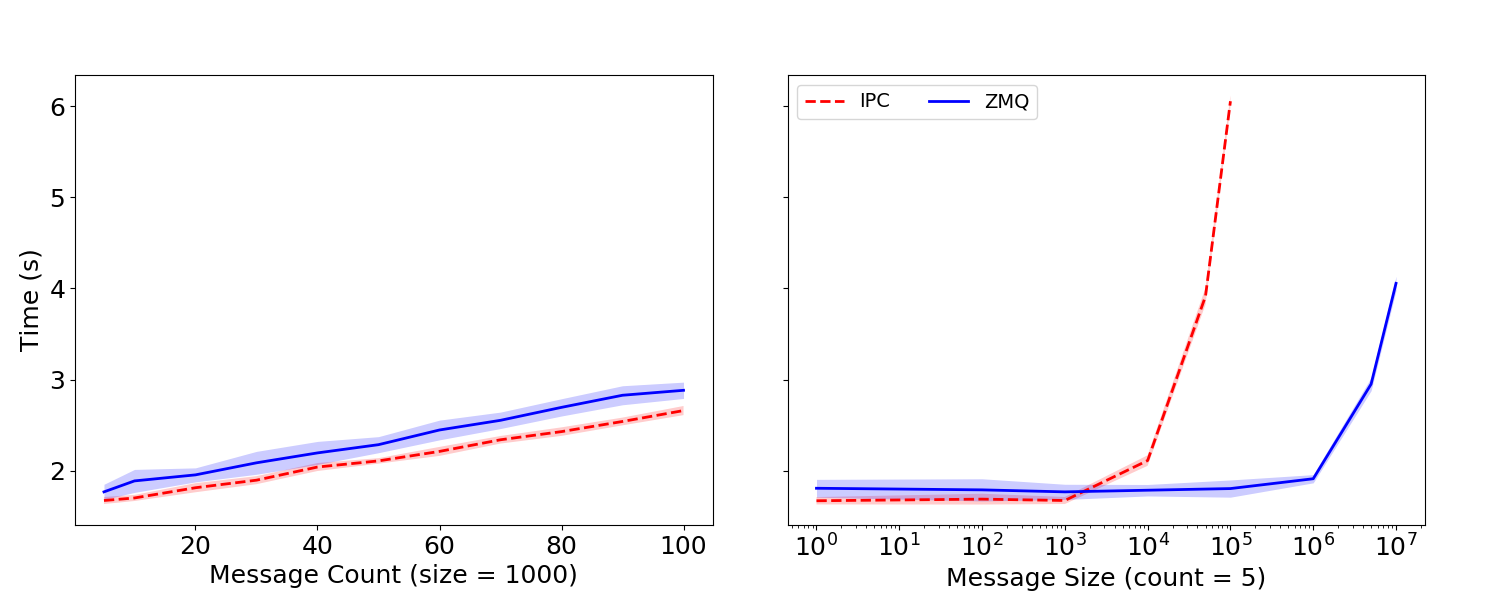
\includegraphics[width=\columnwidth,keepaspectratio]{./images/scaling_commtype.png}
	\caption{Comparison of communication time scaling across communication methods on Linux. Lines show the average run time for each test with the standard deviation shown in the shaded region. Left: Scaling of execution time with number of 1000 byte messages sent. Right: Scaling of execution time with the size of the 5 messages sent.}
	\label{fig:commtype}
	\end{center}
	\end{figure}
\fi
%

Table \ref{tab:commtype} shows how the two communication mechanisms compare as determined by performing a linear fit to the scaling of execution time with message count from Figure \ref{fig:commtype}. Time per message (slope of Figure \ref{fig:commtype}) is the average amount of time required to send a single message containing 1000 bytes and constrains how quickly messages can be passed between the models. Overhead (intercept of Figure \ref{fig:commtype}) is the amount of execution time that would be required if no messages were passed between the models and includes the time required to set up communication mechanisms, start the models, and clean up the integration network.
%
\begin{table}[htbp]
%\caption{The time required per message and overhead for startup/teardown of integration for different communication mechanisms as determined by a linear fit to the scaling of execution time with message count. }
\begin{center}
\begin{tabular}{|c|c|c|}
\hline
Mechanism	& Time per Message (s) 	& Overhead (s) 	\\\hline
IPC			& 0.010				& 1.60			\\
ZMQ 		& 0.012				& 1.73			\\\hline
\end{tabular}
\end{center}
\caption{Effect of communication mechanism on performance.}
\label{tab:commtype}
\end{table}%
%
Although IPC queues are slightly faster than ZMQ TCP sockets in both time per message and overhead for messages smaller than the limit, IPC queues have a much smaller maximum size limit for messages. As discussed in \S\ref{SSS:large}, messages larger than this limit (2048 bytes) must be broken up into multiple messages, compounding the time required to send these messages and making IPC queues a poor choice for sending data over $\sim10^5$ bytes. This limit is much larger for ZMQ sockets ($\sim10^6$ bytes). However, for messages less than the limit, both ZMQ and IPC communication has no measurable dependence on message size.

% LANGUAGE
\subsection{Language}\label{SS:results_language}
%
Figure \ref{fig:language} compares the execution times for integrations with communications between models in different combinations of languages and Table \ref{tab:language} reports the time per message and overhead. The runs for Figure \ref{fig:language} and Table \ref{tab:language} were run on the Linux machine from above while those for Figure \ref{fig:language_matlab} and Table \ref{tab:language_matlab} were run on a 2015 MacBook Pro with a 2.9 GHz Intel Core i5 processor running macOS High Sierra 10.13.4 that had Matlab R2017a installed. In both cases, ZMQ communication was used with Python 2.7.
%
\ifinclfig
 	\begin{figure}[htbp]
	\begin{center}
	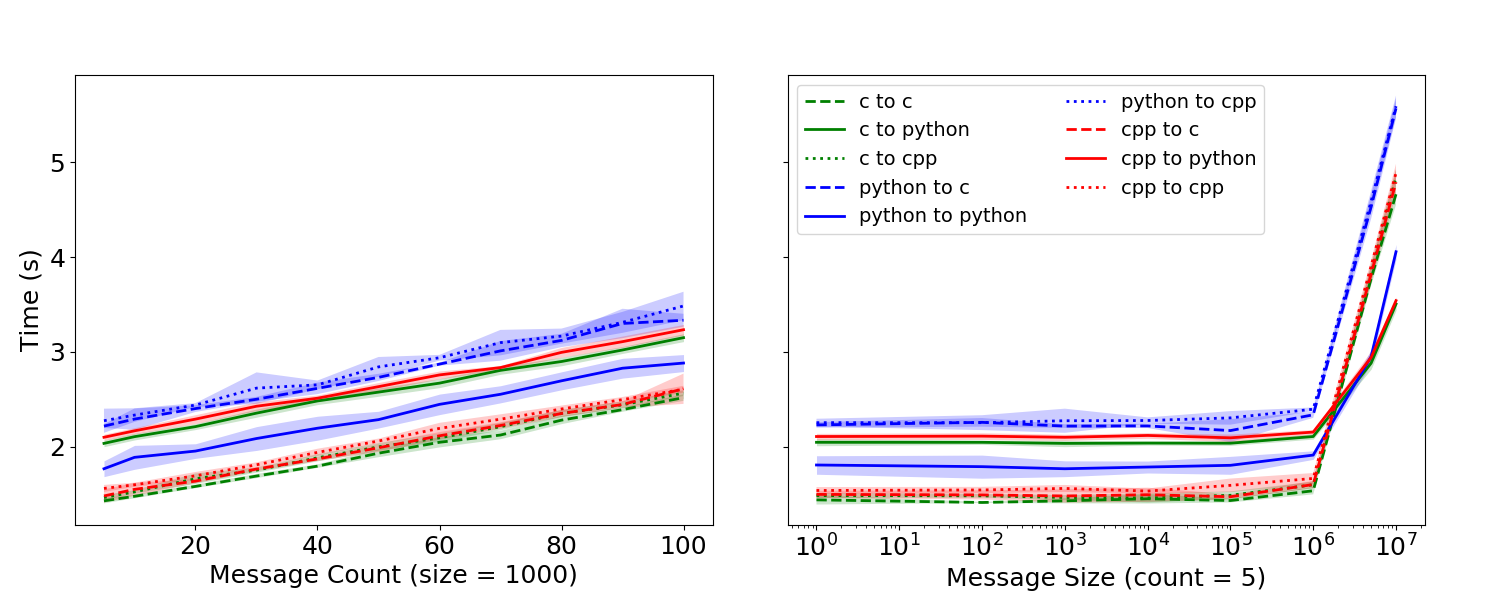
\includegraphics[width=\columnwidth,keepaspectratio]{./images/scaling_language.png}
	\caption{Comparison of communication time scaling between languages on Linux without Matlab. The same fiducial message size (1000 bytes) and count (5) was used as in Figure \ref{fig:commtype}.}
	\label{fig:language}
	\end{center}
	\end{figure}
\fi
%
\begin{table}[htbp]
\begin{center}
\begin{tabular}{|c|c|c|c|}
\hline
Source 	& Destination 	& Time per Message (s) 	& Overhead (s) 	\\\hline
C 				& C					& 0.011				& 1.36			\\
C 				& C++				& 0.012				& 1.42			\\
C 				& Python				& 0.012				& 1.99			\\
\hline%
C++ 				& C					& 0.012				& 1.42			\\
C++ 				& C++				& 0.011				& 1.49			\\
C++ 				& Python				& 0.012				& 2.05			\\
\hline%
Python			& C					& 0.012				& 2.15			\\
Python			& C++				& 0.012				& 2.21			\\
Python			& Python				& 0.012				& 1.73			\\
\hline
\end{tabular}
\end{center}
\caption{Effect of model language on performance (Linux).}
\label{tab:language}
\end{table}%
%
\ifinclfig
 	\begin{figure}[htbp]
	\begin{center}
	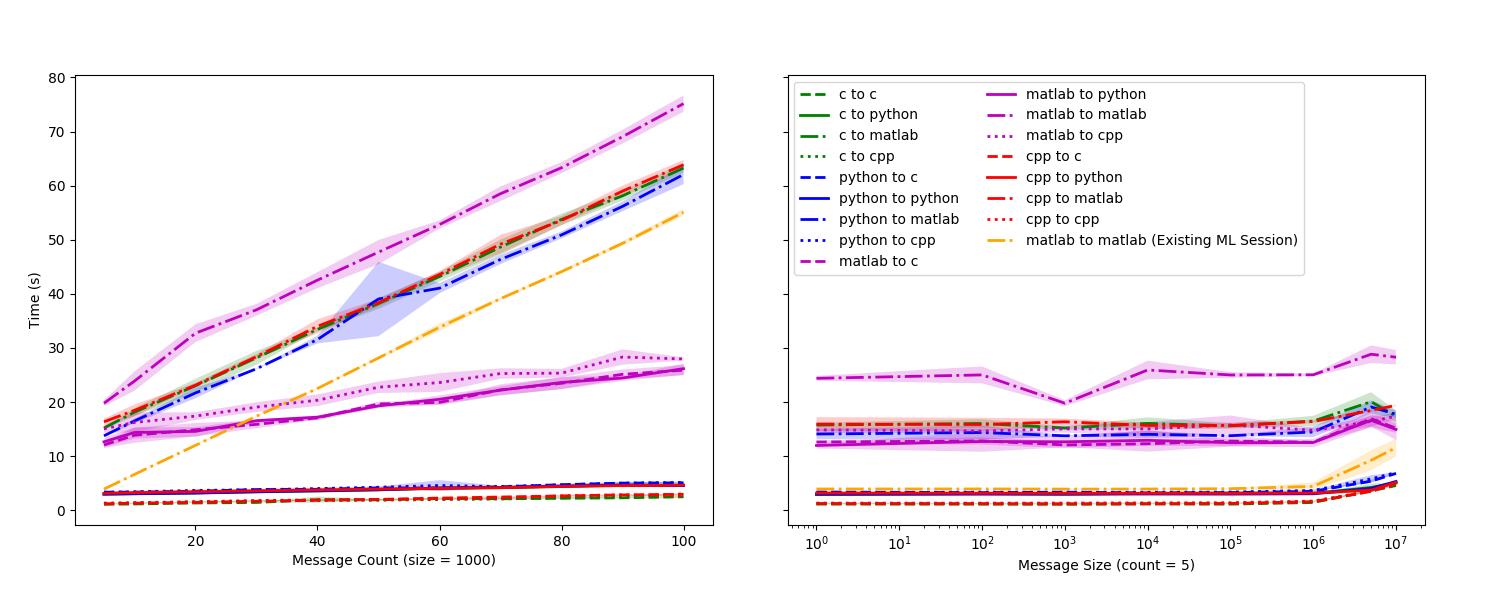
\includegraphics[width=\columnwidth,keepaspectratio]{./images/scaling_language_matlab.png}
	\caption{Comparison of communication time scaling between languages on Mac OS X including Matlab.}
	\label{fig:language_matlab}
	\end{center}
	\end{figure}
\fi
%
\begin{table}[htbp]
\begin{center}
\begin{tabular}{|c|c|c|c|}
\hline
Source 	& Destination 	& Time per Message (s) 	& Overhead (s) 	\\\hline
C 				& C					& 0.015				& 1.11			\\
C 				& C++				& 0.016				& 1.15			\\
C 				& Python				& 0.019				& 2.86			\\
C				& Matlab				& 0.505				& 12.98			\\
\hline%
C++ 				& C					& 0.019				& 1.10			\\
C++ 				& C++				& 0.016				& 1.25			\\
C++ 				& Python				& 0.016				& 3.10			\\
C++ 				& Matlab				& 0.505				& 13.45			\\
\hline%
Python			& C					& 0.019				& 3.17			\\
Python			& C++				& 0.019				& 3.26			\\
Python			& Python				& 0.019				& 2.86			\\
Python			& Matlab				& 0.500				& 11.31			\\
\hline%
Matlab			& C					& 0.144				& 11.82			\\
Matlab			& C++				& 0.142				& 14.79			\\
Matlab			& Python				& 0.139				& 12.23			\\
Matlab			& Matlab				& 0.526				& 21.71			\\
\hline%
Matlab (started)		& Matlab (started)		& 0.537				& 1.25			\\
\hline
\end{tabular}
\end{center}
\caption{Effect of model language on performance (Mac OS X) with Matlab.}
\label{tab:language_matlab}
\end{table}%
%

Except for Matlab models, the time required per message is not affected by the language of either model for smaller messages. There is a very small increase in the time per message when there is a Python model involved, but this is much lower than the standard deviation resulting from background activity on the test machine and so is inconclusive. Matlab models have a much higher time per message than any other language. This results from the way the Matlab interface was implemented, by calling the Python interface. The time required per message is largest when the receiving model is written in Matlab because the receiving models both receives messages from the other model and send output to a file, resulting in twice the number of calls to the wrapped interface. The performance of the Matlab interface may be improved in the future by either implementing it in Matlab directly or by wrapping the C routines.

Language also plays a role for messages larger than the maximum ($2^{20}$ bytes), when messages must be broken into smaller pieces. In particular, integrations that include a C or C++ receiving model scale more strongly than for those that have a Python receiving model because, in addition to the input/output connection drivers, the Python interface itself is asynchronous while the C/C++ interface is not. This means that while Python receiving models have concurrent operations to receive, backlog, and confirm messages, C/C++ models will block on each receive until the input connection driver completes the confirmation handshake. In addition, because C/C++ models are not continuously receiving and backlogging messages, the channel will become saturated. Once it reaches its maximum, the input connection driver can no longer pass along messages and must wait for the model to receive the next message. One remedy that is being explored for future releases, is to make the C/C++ interface asynchronous as well. However, this is a low priority as only models with very rapid and high volume input (such as the test models) are affected.

The largest difference between the different test cases is in in the overhead. Every model language entails some overhead. For interpreted languages (e.g. Python and Matlab), the majority of the overhead comes from starting the interpreter. For Matlab, this is particularly time consuming ($>10$ s). Although this is only a one-time cost required at the start of an integration, {\pkg} does offer ways to alleviate this if multiple runs are necessary by starting a Matlab engine prior to the first integration that can be used by subsequent runs. When Matlab is started in advance (the dashed-dotted orange line in Figure \ref{fig:language_matlab}), the overhead for Matlab models drops to 1.25\,s, less than Python (2.86\,s) but slightly more than C (1.11\,s).

For compiled languages (C and C++), the overhead comes from compiling the source code which is done in serial. The time required for compilation will depend on the compiler used and the complexity of the model code. For command line compiled models, {\pkg} forces the model to be recompiled every time to ensure any changes to the source code are propagated. However, for models that use Make and CMake, overhead due to compile time can be reduced by using existing builds.

Interestingly, the recorded overheads were not symmetric or additive. For example, the Python-to-C integrations required more overhead than the C-to-Python integrations. This is because the models are started in parallel, but do not require the same amount of time to start and being execution. C models, while requiring compilation, start much faster than Python models. In a Python-to-C integration, the C model must wait for the Python model to finish its much slower startup and begin sending message, while in a C-to-Python integration, the C model can immediately begin sending messages that will be received by the Python model once it finishes starting up. In addition, the Python-to-Python integrations required less time than any of the other integrations that included Python because, although Python models take longer to start up, the start up is done in parallel while the compilation for the C and C++ models is done in serial. This source of overhead could be ameliorated by compiling models in parallel or in advanced, but is usually not significant enough to effect overall performance.


% PYTHON VERSION
\subsection{Python Version}\label{SS:results_python}
%
Figure \ref{fig:python} and Table \ref{tab:python} compare the execution times when using different versions of Python. The performance tests for both Python 2.7 and Python 3.5 were performed on the Linux machine from above using ZMQ communication and two different integration (Python-to-Python and C-to-C).
%
\ifinclfig
 	\begin{figure}[htbp]
	\begin{center}
	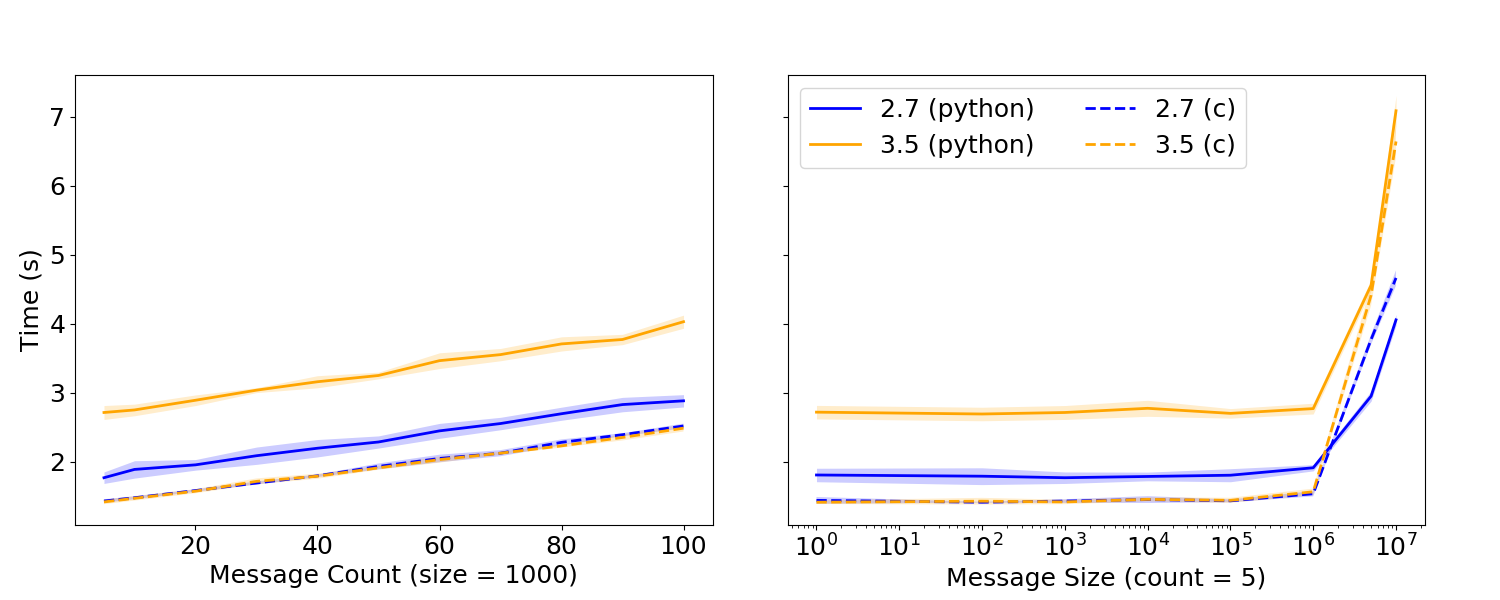
\includegraphics[width=\columnwidth,keepaspectratio]{./images/scaling_python.png}
	\caption{Comparison of communication time scaling between Python versions on Linux. The solid lines are for the Python-to-Python integrations and the dotted lines are for the C-to-C integration.}
	\label{fig:python}
	\end{center}
	\end{figure}
\fi
%
\begin{table}[htbp]
\begin{center}
\begin{tabular}{|c|c|c|c|}
\hline
Python Version	& Language	& Time per Message (s) 	& Overhead (s) 	\\\hline
2.7			& Python		& 0.012				& 1.73			\\
2.7			& C			& 0.011				& 1.36			\\
3.5 			& Python		& 0.013				& 2.62			\\
3.5			& C			& 0.011				& 1.36			\\\hline
\end{tabular}
\end{center}
\caption{Effect of Python version on performance.}
\label{tab:python}
\end{table}          
%
There is $\sim1$\,s additional overhead with Python 3.5 compared to Python 2.7 due to the increased startup time for the Python 3.5 interpreter. This overhead is only present for integrations that include Python models. For comparison, there is no difference in the time per message and overhead between the different Python versions for the C-to-C integration (dashed lines in Figure \ref{fig:python}). There is a slight difference in time per message between the two versions for all models that shows up in the scaling of execution time with message size for large messages ($>10^6$ bytes). Differences at large message sizes between the two versions arrises from the use of Python classes to transport messages between models and is more pronounced in integrations with Python models due to the increased amount of Python code.

% PLATFORM
\subsection{Operating System}\label{SS:results_platform}
%
Figure \ref{fig:platform} and Table \ref{tab:platform} compare the execution times on different operating systems. The performance tests reported for Linux were run on the machine from above. The tests for Mac OS X were run on a 2015 MacBook Pro with a 2.9 GHz Intel Core i5 processor running macOS High Sierra 10.13.4. The tests for Windows were run on the same machine from a dual boot of Windows 10. All platform dependent performance tests use ZMQ communication and the Python-to-Python integration.
%
\ifinclfig
 	\begin{figure}[htbp]
	\begin{center}
	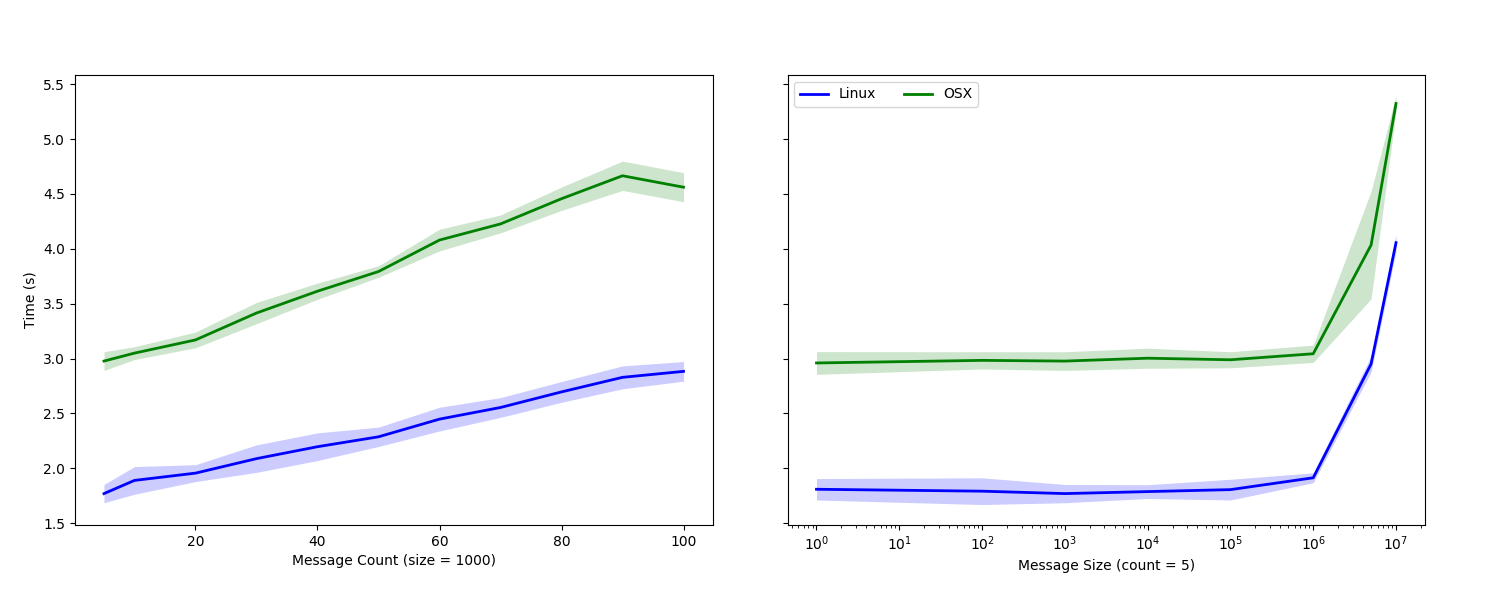
\includegraphics[width=\columnwidth,keepaspectratio]{./images/scaling_platform.png}
	\caption{Comparison of communication time scaling between operating systems.}
	\label{fig:platform}
	\end{center}
	\end{figure}
\fi
%
\begin{table}[htbp]
\begin{center}
\begin{tabular}{|c|c|c|}
\hline
Operating System	& Time per Message (s) 	& Overhead (s) 	\\\hline
Linux			& 0.012				& 1.73			\\
Mac OS X			& 0.019				& 2.86			\\
Windows			& 0.029				& 3.73			\\\hline
\end{tabular}
\end{center}
\caption{Effect of operating system on performance.}
\label{tab:platform}
\end{table}%
%
Both the time per message and overhead changed between operating systems with the Linux machine performing the most consistently and fastest and Windows offering the slowest speeds. Because the Linux test machine was very different from the test machine for both Mac OS X and Windows, it cannot be determined that operating system alone contributed to the observed differences. The same can be said of comparing the Mac OS X and Windows tests given that operating systems are often optimized for their intended hardware. However, the tests do show that {\pkg} performed consistently on each of the supported operating systems.

%---------------------------------------------------------------------------------
% SPEEDUP
\subsection{Speedup from Parallelism}\label{SS:speedup}
%
While efforts have been made to limit the overhead introduced by {\pkg} in the startup and communication steps of the integration, {\pkg} cannot outperform a direct integration of two models if they are tightly coupled and must run sequentially. For example, consider an alternate version of the shoot model from \S\ref{S:example} where the shoot model itself calculates the current root mass, sends the root mass to the root model, and then waits for the response. While the root model is performing the calculation, the shoot model will be idle, waiting for the response and, while the shoot model is calculating the root mass or handling the response, the root model will be idle, waiting for the next input. As a result, such a system will essentially execute in serial, incurring the overhead from using {\pkg} to run the models and coordinate communication without the advantage of parallel execution. Because native language variable passing will always be faster, a direct integration of the two models by translating one into the language of the other will always be faster than the {\pkg} integration in such cases. However, if the two models are not as tightly coupled and have calculations that can occur simultaneously, {\pkg} can offer a significant speedup via parallelism.

Speedup, in the case of parallelism, is defined as the ratio of the serial execution time to the parallel execution time.
%
\begin{equation}
S = \frac{T_{serial}}{T_{parallel}}
\end{equation}
%
For the example presented above of one model (model A) sending output to another (model B) and then waiting for a response, the speedup offered by {\pkg} through parallelism can be parameterized in terms of the durations of calculations for each model performed in the different phases of the process (See Figure \ref{fig:empty_parallel}). 
%
\ifinclfig
 	\begin{figure}[htbp]
	\begin{center}
	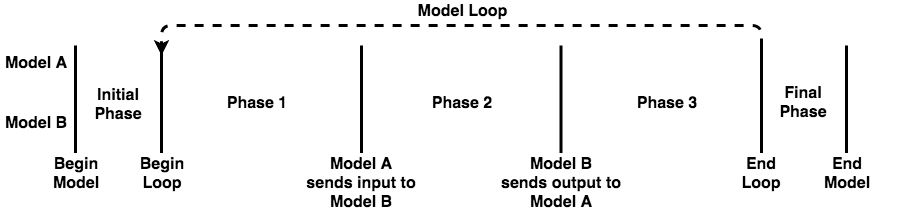
\includegraphics[width=\columnwidth,keepaspectratio]{./images/Parallelism-Empty.png}
	\caption{Diagram of phases in parallel execution of models A (top) and B(bottom). Each model performs some setup actions in the initial phase, enters a loop that contains two communication (first from model A to model B, then from model B to model A), and then performs some teardown actions in the final phase.}
	\label{fig:empty_parallel}
	\end{center}
	\end{figure}
\fi
%
During the initial phase ($t_{init,A}$ \& $t_{init,B}$), both models perform setup tasks before immediately entering the loop. On entering the loop at Phase 1 ($t_{1,A}$ \& $t_{1,B}$), both models perform calculations in preparation for the first communication where Model A sends a message to Model B. In Phase 2 ($t_{2,A}$ \& $t_{2,B}$), Model B processes the message it received and Model A performs actions in preparation for receiving a response during the second communication. In Phase 3 ($t_{3,A}$ \& $t_{3,B}$), Model A analyzes the response and Model B performs any additional calculations needed before the end of the current loop. Following completion of Phase 3 tasks, the models will immediately either enter another loop or enter the final phase ($t_{final,A}$ \& $t_{final,B}$) to complete any necessary cleanup and teardown actions. 
%
If the models in the toy example were run in serial (without {\pkg}), the total execution time would be 
%
\begin{equation}
T_{serial} = t_{init,A} + t_{init,B} + N_{loop}\left[\sum_{i=1}^{3}\left(t_{i,A} + t_{i,B}\right)\right] + t_{final, A} + t_{final, B},
\end{equation}
%
where $N_{loop}$ is the number of loops executed and $t_{x,A}$ and $t_{x,B}$ are the execution times of each phase of the process for models A and B respectively.
%
In order to calculate the parallel execution time, we must consider the effect of asynchronous communication. For every asynchronous call, the receiving model is limited by the sending model, but the sending model is not limited by the receiving model. For a single asynchronous communication between two parallel processes, the execution time will be
%
\begin{eqnarray}
%t_{wait} & = & \max(0, t_{before,sender} - t_{before,receiver}) \\
T_{async} & = & \max\left\{\left[t_{before,send} + t_{after,send}\right], \left[\max(t_{before,send}, t_{before,recv}) + t_{after,recv}\right]\right\},
\end{eqnarray}
%
where $t_{before,send}$ and $t_{after,send}$ are the time the sending model spends in the phases before and after sending the message respectively and $t_{before,recv}$ and $t_{after,recv}$ are the same times, but for the receiving model. The parallel execution time for the example which includes a loop around two asynchronous communications is then a recursive relationship where the execution time for one loop depends upon the relative execution times of the two models for the previous loop. This relationship can be written as a recursive formula
%
\begin{equation}
T_{parallel} = T_{overhead} + \max(T_{A,N_{loop}}, T_{B,N_{loop}}),
\end{equation}
\begin{equation}
\begin{cases}
T_{A, 0} = t_{init,A} + t_{final,A} \\
T_{A, n} = \max\left[(T_{A, n-1} + t_{comm} + t_{1,A} + t_{2,A} - t_{final,A}), (T_{B, n} - t_{3,B} - t_{final,B})\right] + t_{3,A} + t_{final,A}\\
T_{B, 0} = t_{init,B} + t_{final,B}\\
T_{B, n} = \max\left[(T_{B, n-1} + t_{comm} + t_{1,B} - t_{final,B}), (T_{A, n-1} + t_{1,A} - t_{final,A})\right] + t_{2,B} + t_{3,B} + t_{final,B}\\
%3x + 5y + z \\ 7x ? 2y + 4z \\ -6x + 3y + 2z 
\end{cases}
\end{equation}
%
where $T_{overhead}$ is the overhead incurred by using {\pkg} to run the models and setup the communication network, $t_{comm}$ is the time required to complete the exchanges via each {\pkg} asynchronous communication, $n$ is the number of loops, and $T_{A,n}$ and $T_{B,n}$ are the times required by each model to complete their individual task in parallel for the given number of loops. While $T_{overhead}$ and $t_{comm}$ can be determined from the previous results sections for a given set of languages, the other variables are entirely dependent on the speed of the code occupying each phase. This relationship can also be written more intuitively as an algorithm (See Algorithm \ref{alg:tpara}) 
%
% tA = tinitA
% tB = tinitB
% iloop = 0
%
% WHILE (iloop < nloop)
%	tA += t1A
%	tB += t1B
%	# FIRST LOCK
% 	IF tB <= tA: B waits for A at Lock 1 and they are synchronized
%		tB = tA
%	tA += t2A
%	tB += t2B
%	# SECOND LOCK
%	IF tA <= tB: A waits for B at Lock2 and they are synchronized
%		tA = tB
%	tA += t3A
%	tB += t3B
%	iloop++
% tA += tfinalA
% tB += tfinalB
% Tpara = max(tA, tB)
%
\begin{algorithm}[H]
    \caption{Parallel Execution Time}
    \label{alg:tpara}
    \begin{algorithmic}[1] 
    \State $T_{A} \gets t_{init,A}$
    \State $T_{B} \gets t_{init,B}$
    \State $iloop \gets 0$
    \While{$iloop <= N_{loop}$}
    	\State $T_{A} += t_{1,A}$
	\State $T_{B} += t_{1,B}$
	\State $T_{B} = \max(T_{A}, T_{B} + t_{comm})$ \Comment{Model B blocking on receive.}
	\State $T_{A} += t_{2,A}$
	\State $T_{B} += t_{2,B}$
	\State $T_{A} = \max(T_{A} + t_{comm}, T_{B})$ \Comment{Model A blocking on receive.}
	\State $T_{A} += t_{3,A}$
	\State $T_{B} += t_{3,B}$
	\State $iloop += 1$
    \EndWhile
    \State $T_{A} += t_{final,A}$
    \State $T_{B} += t_{final,B}$
    \State $T_{parallel} = \max(T_{A}, T_{B})$
    \end{algorithmic}
\end{algorithm}
%
If the models are completely dependent on one another such that neither has any calculations to perform while the other is working, the situation would be that shown in Figure \ref{fig:serial}. 
%
\ifinclfig
 	\begin{figure}[htbp]
	\begin{center}
	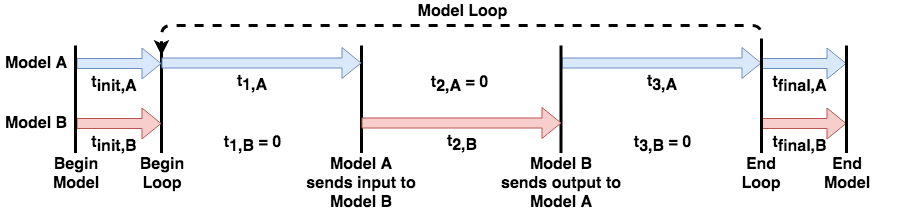
\includegraphics[width=\columnwidth,keepaspectratio]{./images/Parallelism-Serial.png}
	\caption{Diagram of parallelism for a fully coupled set of models. The shaded arrows represent active calculation by models A (top) and B(bottom). Absence of an arrow indicates idle time where the model process is not performing any calculations.}
	\label{fig:serial}
	\end{center}
	\end{figure}
\fi
%
Assuming that $t_{init,B} < (t_{init,A} + t_{1,A})$, this integration would have a parallel execution time and speedup of
%
\begin{eqnarray}
T_{parallel} & = & T_{overhead} + N_{loop}(t_{comm} + t_{1,A} + t_{2,B} + t_{3,A}) + \max\left[(t_{init,A} + t_{final,A}), (t_{init,B} + t_{final,B})\right] \\
S & = & \frac{t_{init,A} + t_{init,B} + N_{loop}(t_{1,A} + t_{2,B} + t_{3,A}) + t_{final, A} + t_{final, B}}{T_{overhead} + N_{loop}(t_{comm} + t_{1,A} + t_{2,B} + t_{3,A}) + \max\left[(t_{init,A} + t_{final,A}), (t_{init,B} + t_{final,B})\right]}
\end{eqnarray} 
%
If the initial and final phases require an insignificant amount of time in comparison with the time spent in the loop, this will approach a speedup of 1, indicating that there was no change in the execution time. However, due to the required overhead ($T_{overhead}$) and communication times ($t_{comm}$) incurred by a {\pkg} integration, it is more likely that the speedup will be below 1 in such a case unless the calculations have a long enough duration to render these costs inconsequential. For example, if we consider two Python models ($t_{comm} = 0.02$\,s/msg and $T_{overhead} = 2.86$\,s) where $t_{1,A}$, $t_{2,B}$, and $t_{3,A}$ are all 1\,s with initial and final phases that are 0.1\,s for both models, the speedup will be 0.92 for 10 loops and 0.99 for 100 loops.

If the models are perfectly matched in that each spends exactly the same amount of time in each phase ($t_{init,A}=t_{init,B}$, $t_{1,A}=t_{1,B}$, etc.) as in Figure \ref{fig:parallel},
%
\ifinclfig
 	\begin{figure}[htbp]
	\begin{center}
	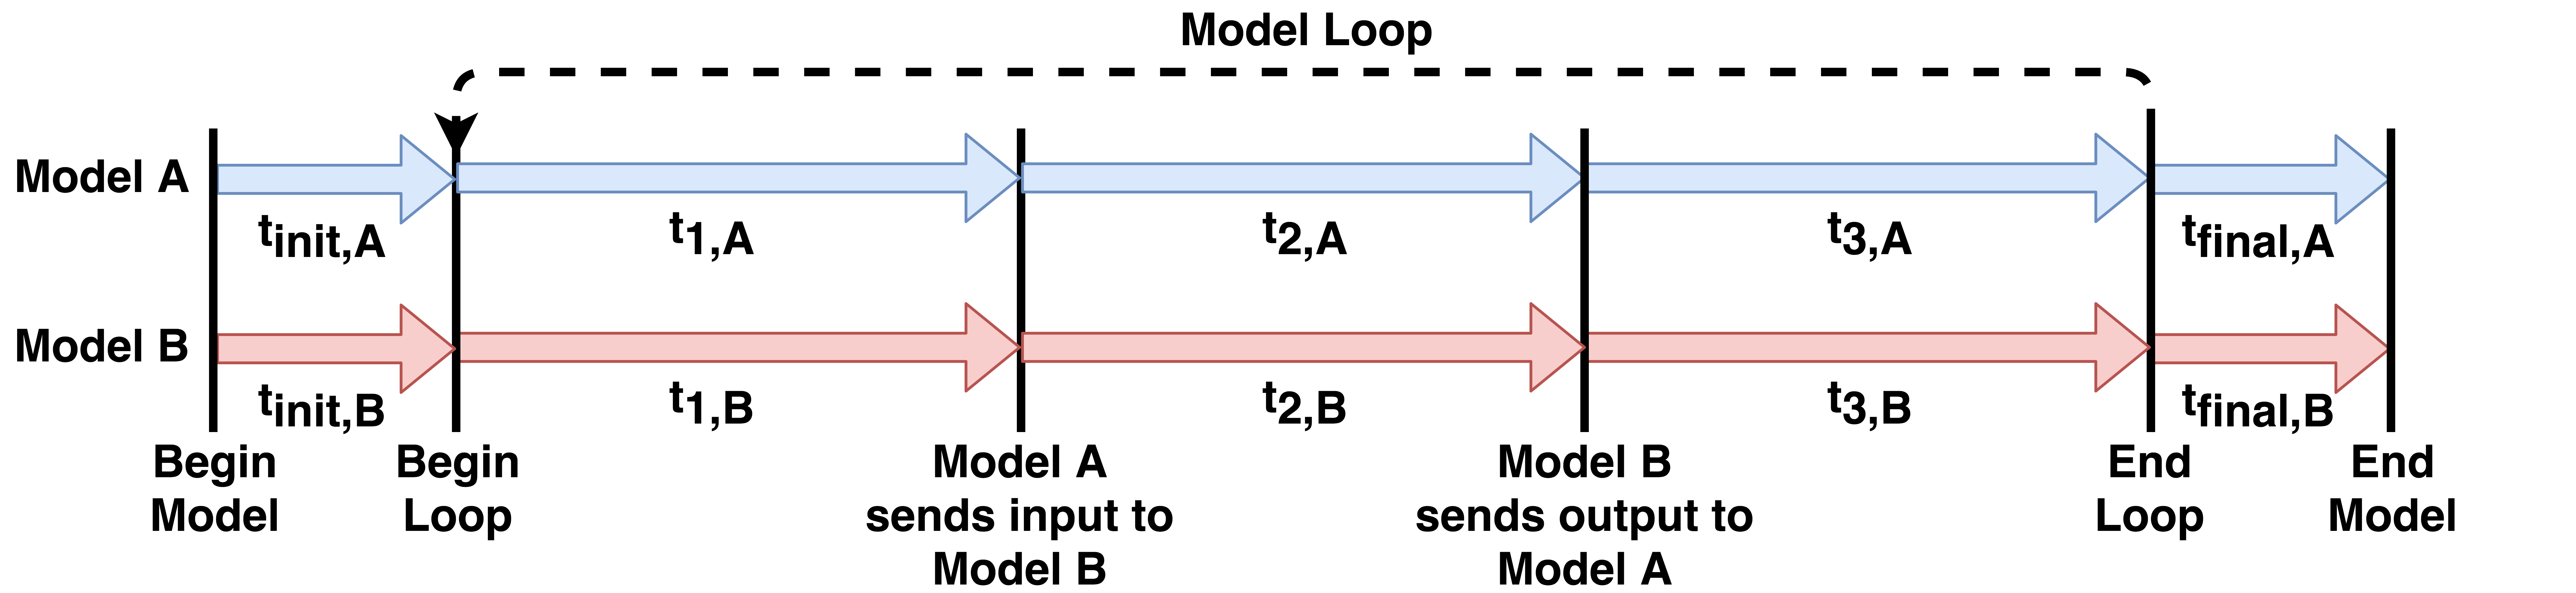
\includegraphics[width=\columnwidth,keepaspectratio]{./images/Parallelism-FullyParallel.png}
	\caption{Diagram of parallelism for a set of perfectly matched models.}
	\label{fig:parallel}
	\end{center}
	\end{figure}
\fi
%
the parallel execution time and speedup of the integration would be
%
\begin{eqnarray}
T_{parallel} & = & T_{overhead} + t_{init,A} + N_{loop}\left(t_{comm} + \sum_{i=1}^{3}t_{i,A}\right) + t_{final, A} \\
S & = & \frac{2\left[t_{init,A} + N_{loop}\left(\sum_{i=1}^{3}t_{i,A}\right) + t_{final, A}\right]}{T_{overhead} + t_{init,A} + N_{loop}\left(t_{comm} + \sum_{i=1}^{3}t_{i,A}\right) + t_{final, A}}.
\end{eqnarray} 
%
If the runtime is sufficiently long such that contributions from $T_{overhead}$ and $t_{comm}$ become insignificant, the speedup will approach 2, the maximum for two processes. For example, if we consider two Python models ($t_{comm} = 0.02$\,s/msg and $T_{overhead} = 2.86$\,s) where both models have Phases 1-3 of 1\,s in duration and initial and final phases of 0.1\,s in duration, the speedup will be 1.82 for 10 loops and 1.97 for 100 loops.

However, the situations shows in Figures \ref{fig:serial} and \ref{fig:parallel} are rarely the case for actual models. Figure \ref{fig:partial} shows a more realistic case in which the models have some overlapping operations, but are not perfectly aligned. 
%
\ifinclfig
 	\begin{figure}[htbp]
	\begin{center}
	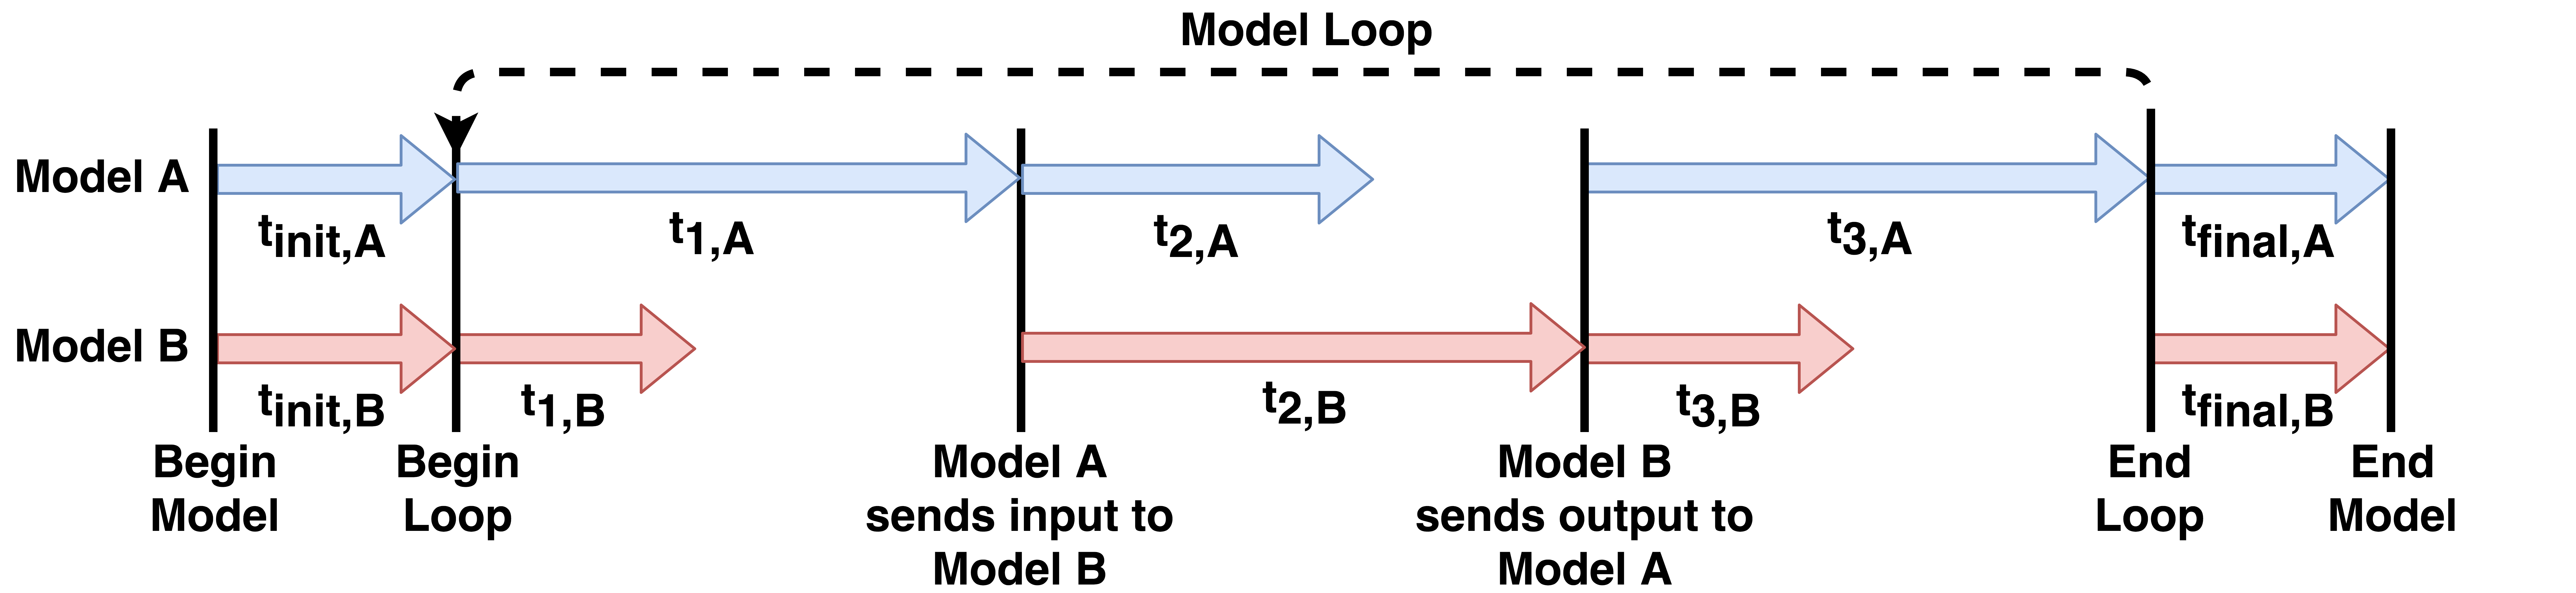
\includegraphics[width=\columnwidth,keepaspectratio]{./images/Parallelism-PartiallyParallel.png}
	\caption{Diagram of partial parallelism for a set of imperfectly matched models.}
	\label{fig:partial}
	\end{center}
	\end{figure}
\fi
%
Speedups in such cases would be between 1 and 2. For example given the parameters shown in Table \ref{tab:partial} for two Python models ($t_{comm} = 0.02$\,s/msg and $T_{overhead} = 2.86$\,s), the speedup will be 1.38 for 10 loops and 1.49 for 100 loops.
%
\begin{table}[h]
\caption{Speedup calculation example parameters for a set of imperfectly matched models.}
\begin{center}
\begin{tabular}{|l|c|c|}
\hline
Phase 	& Duration in Model A (s) & Duration in Model B (s) \\\hline
initial		& 0.1 	& 0.2 \\
1		& 1.0		& 0.3 \\
2		& 1.2		& 2.0 \\
3		& 0.1		& 0.05 \\
final		& 0.1		& 0.1 \\
\hline
\end{tabular}
\end{center}
\label{tab:partial}
\end{table}%
%

For more complex integration involving more than 2 models or more than 2 communications per loop, speedup calculations will be more complex. In general, the maximum possible speedup will be greater for integrations of models that are more independent, but wrappers can be adjusted to deliberately perform tasks during periods where a model would be waiting for a message in order to get greater performance boosts.


%---------------------------------------------------------------------------------
%---------------------------------------------------------------------------------
% SUMMARY & DISCUSSION
\section{Summary}\label{S:discuss}

%---------------------------------------------------------------------------------
% CURRENT STATUS
\subsection{Current Status}\label{SS:current}
%
{\pkg} is an open-source Python package for connecting computational models across programming languages and scales to form integration networks. Models are run in parallel with asynchronous message passing handled under-the-hood via threading and one of three communication mechanisms. {\pkg} works on Linux, Mac OS X, and Windows operating systems with Python 2.7, 3.4, 3.5, 3.6 and 3.7. {\pkg} currently supports running models written in Python, C, C++, and Matlab with additional support for compiling models C/C++ using Make \citep{Stallman2004} or CMake \citep{Martin2006} and running models written in the LPy \citep{Boudon2012} DSL.

%is unique as a framework in several respects:
%\begin{itemize}
%	\item Asynchronous communication via 3 different communication mechanisms. 
%	\item Create and coordination of asynchrnous communication networks that 
%\end{itemize}

{\pkg} is designed to make models as reusable as possible. Once integrated via {\pkg}, models can be combined with any other models that also have a {\pkg} wrapper and YAML specification file with minimal, if any, modification. This "plug-and-play" approach to models encourages model writers to make their codes public in a reusable form, generating citations and reuse of their work, while also growing a community of models and model writers capable of probing areas otherwise unreachable. 
%Generic workflow, parallelization, and communication tools can be used to expose/connect models, but without a standard for making connections, every new integration will require a great deal of hands on attention and new code. Domain specific frameworks like OpenAlea \citep{Pradal2008} are better for improving the reusability for some models in that they can impose a standard for how models interact with each other, however none of the existing frameworks offer the same flexibility as {\pkg} in terms of languages with native support and model form.
%Integration via {\pkg} requires minimal modification of the existing model source code yet greatly increases the model's potential by allowing it to be reused in combination with other models. 
%
{\pkg} has already been used to integrate several plant models within the Crops in Silico organization \citep{Marshall-Colon2017} with ongoing work to add additional models to the integration network. Figure \ref{fig:network} shows the progress so far. 
%
\ifinclfig
 	\begin{figure}[htbp]
	\begin{center}
	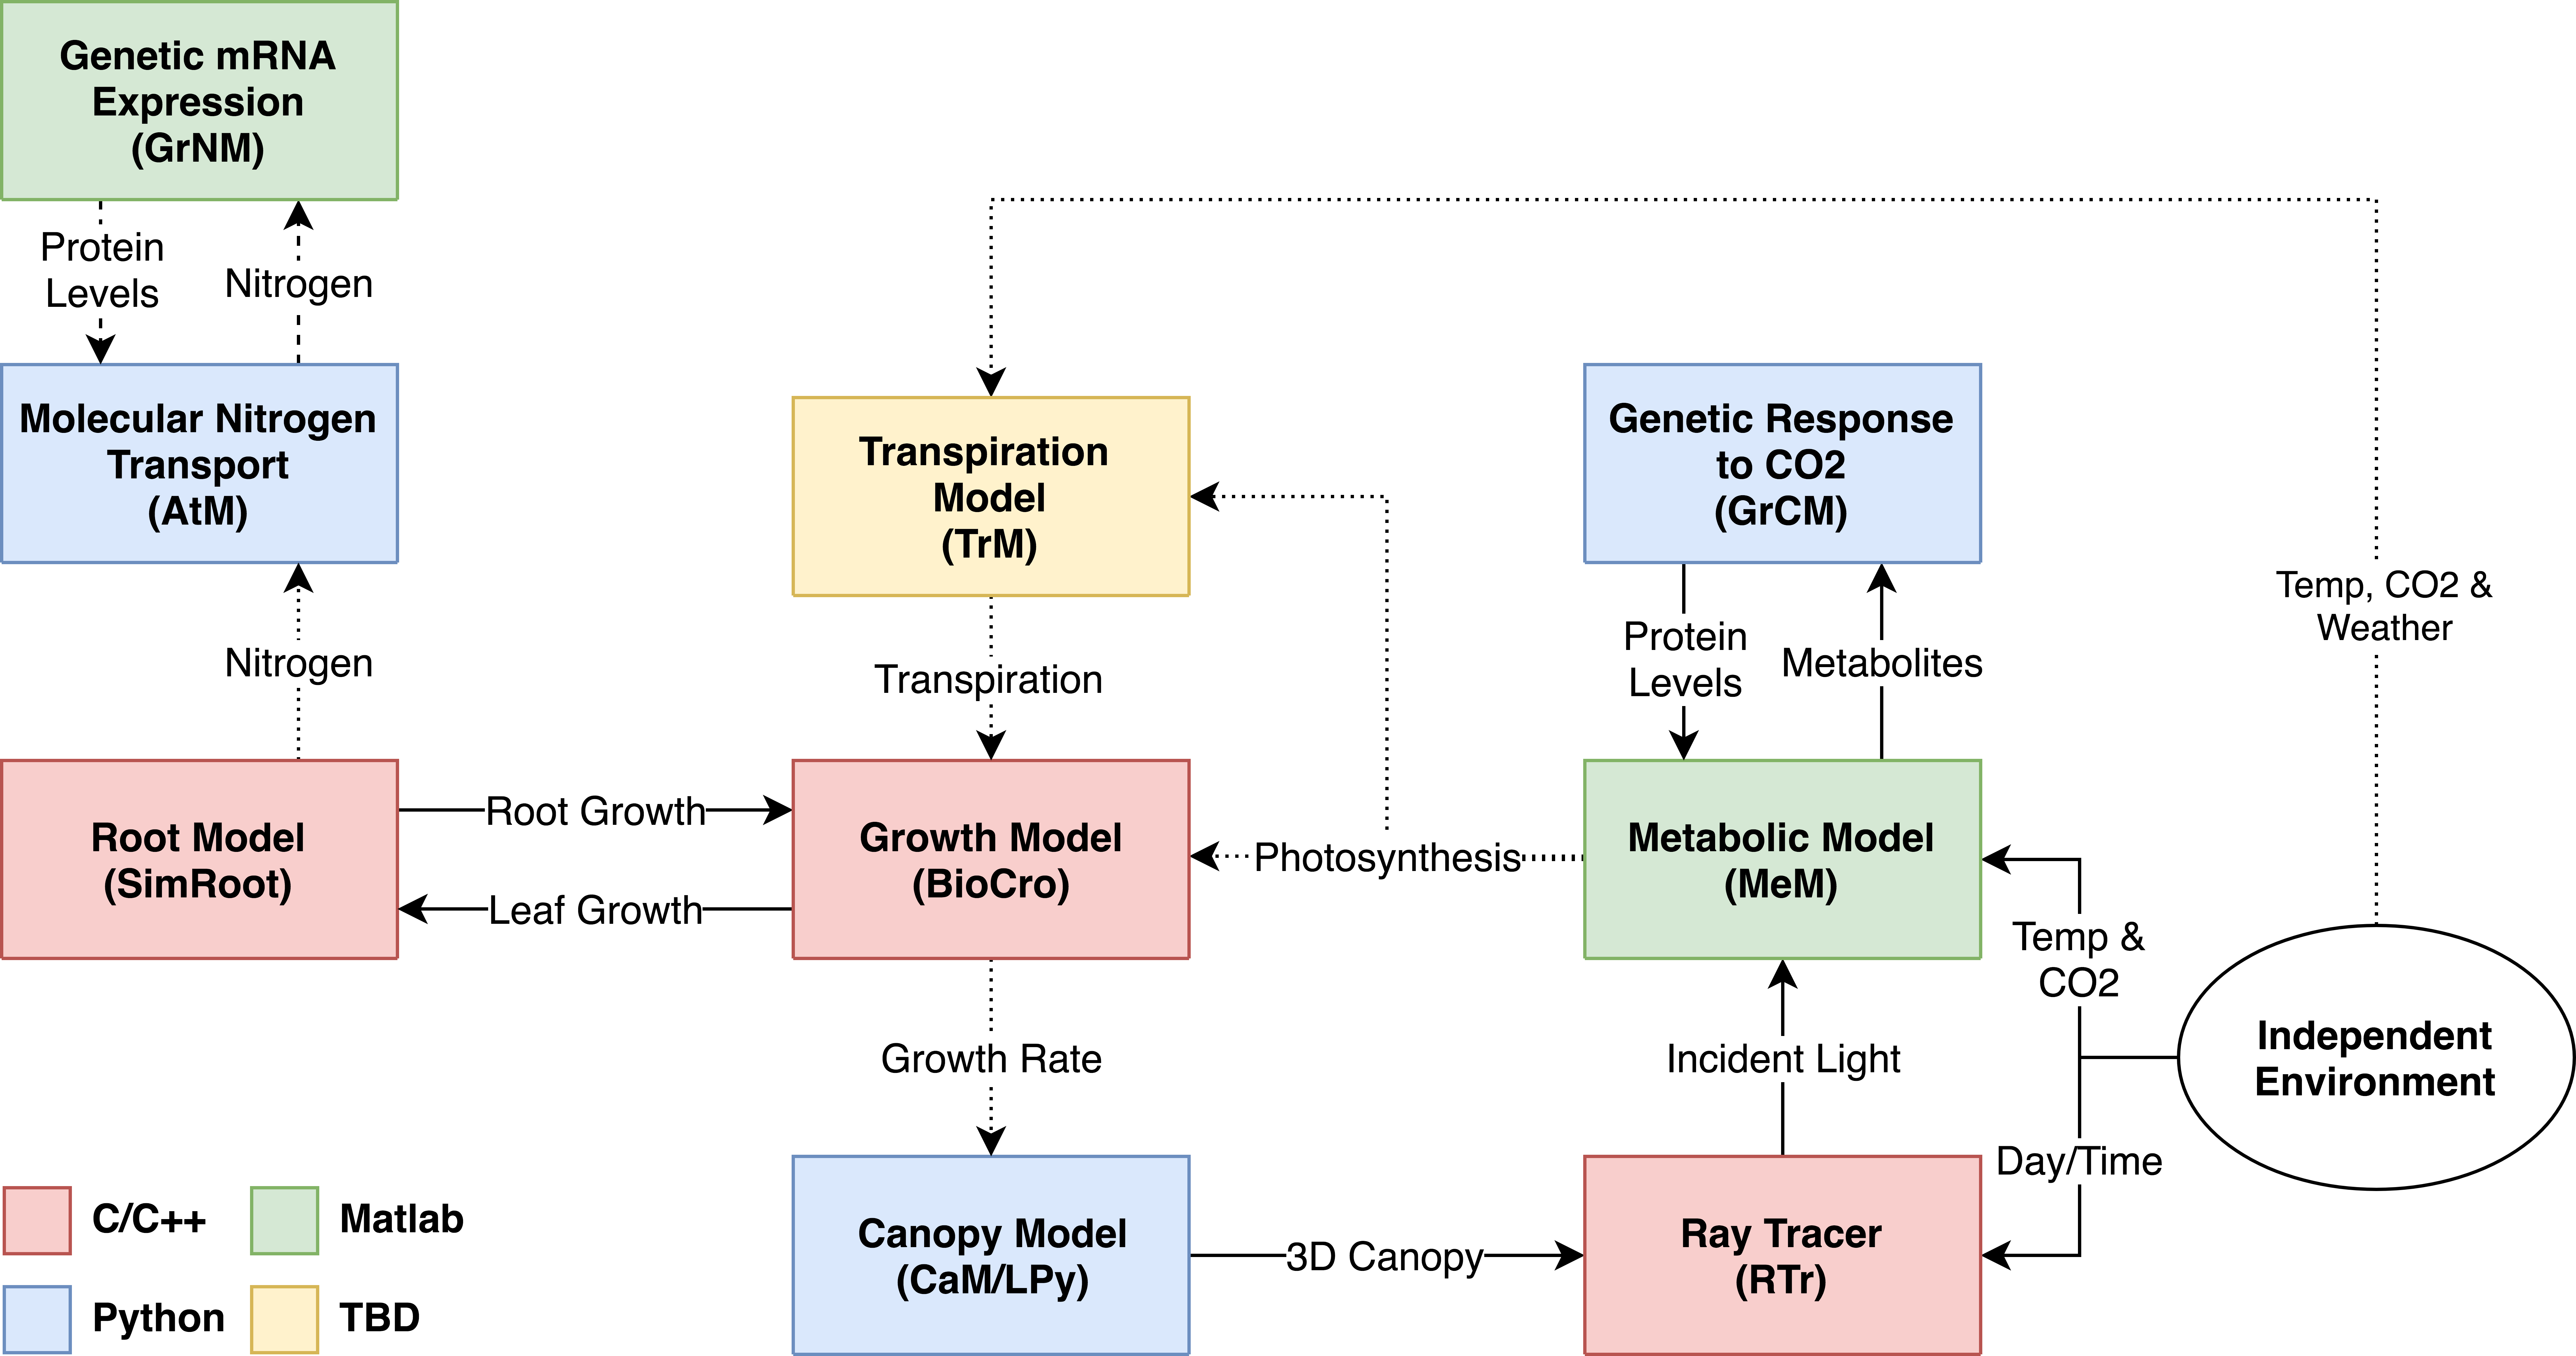
\includegraphics[width=\columnwidth,keepaspectratio]{./images/CiS-Languages.png}
	\caption{Progress towards full Crops in Silico integration network. Each square represents a model and the color of the square indicates the language in which the model is written. Arrows between models represent connections being made between the models using {\pkg}. Solid lines are connections that have already been made, dashed lines are in-progress connections, and dotted lines are planned connections.}
	\label{fig:network}
	\end{center}
	\end{figure}
\fi
%
Each square is a model, color indicates the programming language that the model is written in, and lines between the models represent connections where information is exchanged. Solid lines are connections that have already been implemented, dashed lines are connections currently being implemented, and dotted lines are connections planned for the future. When complete, the integration network will include 9 models of molecular, genetic, cellular, organ, and plant level processes in 4 different programming languages, produced by $>10$ researchers at 4 different institutions. 

Although not yet complete, partial integrations from this network are already yielding new insights. For example, by integrating a metabolic flux model  with gene expression data from soybean (\emph{Glycine max}) plants grown under ambient (380\,$\mu$mol/mol) and elevated (550\,$\mu$mol/mol) carbon dioxide (CO$_2$), 
%
\ifieee
	\citep{integration_prep} 
\else
	\citet{integration_prep} 
\fi
%
simulated the increased carbon assimilation rate observed in field studies \citep{Bernacchi2005}. The integrated modeling also identified gene candidates predicted to regulate enzymes involved in the light and dark reactions of photosynthesis under elevated CO$_2$.

In addition to allowing scientists to reuse existing models in new integrations and make new connections, {\pkg} has the potential to significantly increase a model's accessibility and promote reuse. {\pkg} could be used as a method of running models without knowledge of the model's implementation. At publication, model code could be released along with a wrapper and YAML specification file for use with {\pkg}. These additional materials would be particularly powerful when considered alongside the interactive features being developed for use with {\pkg} (see \S\ref{SS:gui} and \S\ref{SS:function}). Potential collaborators could use {\pkg} to run and explore models without the need to be familiar with the inner workings of the model implementation or even implementation language.

%---------------------------------------------------------------------------------
% USE CASES AND LIMITATION
%
\subsection{Advantages \& Limitations}\label{SS:uses}
%
\subsubsection{Advantages}\label{SS:advantages}
%
{\pkg} offers several advantages over manual integrations or other existing tools.
%
\begin{description}
	\item[Dynamic Communication Network] While there are many existing tools for communication that have implementations in multiple languages \citep[some of which {\pkg} uses, e.g.][ZMQ, RabbitMQ, OpenMPI]{ZMQ, RMQ, Gabriel2004}, these tools require that the communication pattern be well established such that it can be hard coded into the model (or model wrapper) itself (e.g. using specific ports or queues). The use of hard coded values greatly restricts the reusability of a model. For every integration a model is used in, the hard coded values for every connection must be updated between the models on either end so that they match. {\pkg} is unique in that it dynamically establishes and manages the networks of communication resources (e.g. queues, channels, sockets) that are required for integrations to run so that models do not need to have these hard coded value and can be reused in multiple integrations, unmodified. This process includes creating new resources, connecting to existing resources, passing the appropriate resource addresses to the model environment, error handling/propagation, and resource cleanup. 
	\item[Hands-off Parallelism \& Asynchronous Communication] In addition to inter-language communication, {\pkg} users benefit from speedups due to parallelism and concurrency without any additional work. From the specified model connections, {\pkg} manages the parallel execution of models and asynchronous message passing under-the-hood so that the user doesn't have to think about it. Existing tools for asynchronous communication between unmanaged parallel tasks \citep[e.g. Jack2,][]{Magoules2018} requires explicit definition of the communication pattern in advance, prohibiting dynamic communication networks as discussed above. Work/data flow tools like Parsl \citep{babuji18} allow dynamic execution of processes along a dependency chain in parallel, but usually require additional code, are limited to passing data as files or data object native to the tool's implementation language, and are ill-suited to models with persistent internal states or intermediate communication. {\pkg} is unique in that it offers users asynchronous communication and parallelism that is flexible enough to support any communication pattern, implicitly handles conversion between native data types in the supported languages, and does not require any additional time investment on the part of the user to achieve a speedup.
	\item[No New Language] Unlike DSLs or language specific frameworks, {\pkg} doesn't require a model to be written in one specific language. In addition to expanding the possible number of model combinations, this eases the burden on model writers for whom learning an additional programming language or DSL might be a significant obstacle. {\pkg} is designed such that model writers only need to be familiar with the language that the model is written in to being with. Although {\pkg} is a Python package, users do not even need to be familiar with the Python language and can interact with {\pkg} solely through the command line. While users do need to be able to compose YAML specification files in addition to their model code, these files have a very limited syntax and will be GUI composable in future releases.
\end{description}

\subsubsection{Limitations}\label{SS:limitations}
%
While {\pkg} is a powerful tool for integrating scientific models and opening up new avenues for collaboration, it is not applicable to every scenario. Before diving into model integration, potential users should determine if their use case falls under one of the following scenarios.
%
\begin{description}
	\item[Single Language Integrations] For models written in the same language, it is usually much more computationally efficient to either integrate the models directly (i.e. by calling one from the other) or use a language specific tools for parallel execution and passing data \citep[e.g. Parsl in Python][]{babuji18} than to use {\pkg}. This performance advantage will be particularly pronounced for models that finish quickly or tightly coupled integrations where models make a large number of exchanges in rapid succession (e.g. a set of coupled ODEs). Although the constituent models will still benefit from integration via {\pkg} in regards to reusability, {\pkg} may not be the best choice in such cases if execution time is a concern. Future work on automated creation of wrapper files for function-like (\S\ref{SS:control}) and ODE (\S\ref{SS:ODE}) models may allow {\pkg} to handle this automatically, replacing managed communication with in-language variable passing for models that are written in the same language and co-located on the same machine.
	\item[Fast \& Tightly Coupled Models] For models involving quick calculations or for tightly couple sets of models such as might occur for two models representing coupled ODEs, the computational cost of rapid communication via {\pkg} can quickly surpass the cost of the calculations themselves causing the {\pkg} to be computationally inefficient in comparison with a manual integration. For example, if the sleep statements were removed from the example root and shoot models from \S\ref{S:example}, the calculations become trivial and take significantly less time than the communication between the models. Without the sleep statements, the root and shoot models run for 100 time steps in 0.007\,s and 0.095\,s respectively while the integration takes 7.437\,s. The speedup offered by {\pkg} is then 0.0137, which is actually a \emph{significant} slow down. For such models, large parameter searches or integrations with many time steps can be computationally prohibitive with {\pkg}.
	\item[Unsupported Languages] While {\pkg} currently supports models written in Python, Matlab, C, \& C++, these languages are not an exhaustive list of those languages in which models are written. There are plans to expand support for {\pkg} to other languages (see \S\ref{SS:langsupport}), but in the meantime {\pkg} will not be particularly useful for models that are not written in one of the languages already supported. However, if a language can be called from one of the supported languages or vice versa \citep[e.g. f2py or SWIG,][]{Peterson2009,Beazley2003}, it may be possible to either write a wrapper or make calls to an interface in a supported language.
\end{description}

%---------------------------------------------------------------------------------
% FUTURE WORK
\subsection{Ongoing/Future Improvements}\label{SS:future}
%
{\pkg} is being actively developed to expand the number of models that can be used in integration networks and the complexity of integration networks that can be executed. Several improvements are already in progress/planned for {\pkg}.

% LANGUAGE SUPPORT
\subsubsection{Language Support}\label{SS:langsupport}
%
The biggest barrier to running new models is language support as plant models are written in many different languages. While the current language support covers many of the most popular languages among plant biologists, additional languages must be added to unlock the full set of potential integrations. Informal surveys of the plant modeling community during recent conferences and workshops have helped identify the core languages being used by model developers that would have the larges impact on the number of models accessible via {\pkg}. Based on these results, we plan to expand {\pkg} to support models written in R, Fortran, Java, and the SBML \citep{Hucka2003} DSL during the next major development push with support for additional models in subsequent releases as requested.

We also plan to add support for running Matlab models using Octave \citep{Eaton2002}. Matlab models require a Matlab license to run. Given that plant modelers do not all use Matlab, it cannot be assumed that everyone will have access to a Matlab license. Octave is open source and provides much of the same functionality as Matlab and can run many Matlab codes. Support for Octave will improve modelers ability to collaborate without worrying about access to a Matlab license. 

% DISTRIBUTED SYSTEMS
\subsubsection{Distributed Systems}\label{SS:distributed}
%
High performance computing (HPC) and cloud compute resources are powerful tools in the current computing ecosystem that could be used for running complex integration networks. To this end, we plan to expand {\pkg} support for running integration networks on distributed compute resources. {\pkg} already uses communication tools that can be adapted for use in a distributed pattern \citep[ZMQ, RMQ][]{ZMQ, RMQ} and we will leverage tools like the libsubmit package from the Parsl project \citep{babuji18} for automating the submission process to HPC and compute resources. This work will also enable {\pkg} to adaptively spawning additional model processes on elastic compute resources when a model becomes a bottle neck to the integration process. This feature will be particularly useful for integrations simulating large ensembles of biological units (e.g. leaves on a plant or plants in a field) and will enable scientists to explore emergent properties of these systems.

In addition, we will also add tools to {\pkg} for running models as a service and using RMQ to permit access to these models within integration networks. This feature will be useful for scientists who are unable or unwilling to share the source code for their model. Instead, these models can be hosted on dedicated compute resources managed by the model's home institution and collaborators interested in using the model in an integration can connect to it remotely, submitting requests and receiving results as needed.

% CONTROL FLOW
\subsubsection{Wrapper Automation \& Control Flow}\label{SS:control}
%
Currently, modelers must explicitly decide how a model will be used when writing the model wrapper. These decisions can include things like which input and output variables are static versus variable, if there are sets of variables that should be updated at the same time, and how often output is generated, resulting in a hard coded use pattern. If someone wishing to use the model in another integration requires a different use patter, they will need to write their own wrapper. However, for models that have a functional form, the process of writing the model wrapper can be automated and done dynamically for each integration. We plan on adding options to {\pkg} for dynamically generating model wrappers based a user provided function call and list of static/variable input channels. This feature will improve the reusability of model code such as during parameter studies and decrease the amount of work required for integrating models that are written or can be exposed in a functional form. 

Dynamic generation of model wrappers also opens up possibilities for managing the flow of data through an integration network from the YAML. As part of the wrapper automation feature, we will add options for users to specify conditional execution of models via the YAML specification file. For example, a user may have two models for the same process that are valid under different conditions. This feature will allow users to declare this conditional in the YAML such that {\pkg} automatically switches between the two models as appropriate without the need to write an additional wrapper encoding the conditional.

%Control flow and wrapper automation will be part of the {\pkg} 1.0 release.

% ODE
\subsubsection{Symbolic ODE Models}\label{SS:ODE}
%
Many biological models can be posed as a series of coupled ordinary differential equations \citep[ODEs, ][]{WANG2015}. The equations describing such models can be easily formulated into symbolic representations \citep[e.g. SymPy][]{Meurer2017} with well defined inputs and outputs that can be solved by existing tools designed specifically for that task \citep[e.g. scipy.integrate.ode][]{Jones2001, Hairer1993}. Using these tools, we will add features to {\pkg} that allow ODE models to be constructed directly from symbolic representations provided in YAML specification files. These features will allow users to quickly prototype new models and integrate old ones without the need to write a wrapper.

Symbolic integration of ODE based models also has advantages for performance. Integrating models containing coupled ODEs is currently one of the hardest problems for {\pkg} to tackle due to the performance cost associated with rapid communications between models (see \S\ref{SS:limitations}). However, symbolic ODE representations can be used to represent two coupled ODE models as a single model which is much more computationally efficient as it does not require communication via {\pkg}. As such, ODE support for {\pkg} will also include automated coupling at runtime such that, while two ODE models can be declared separately and used independently in integrations, they will be combined into a single code when connected. This feature will greatly improve the performance of {\pkg} for integration of coupled ODEs.

% DATA AGGREGATIOIN
\subsubsection{Data Aggregation \& Forking}\label{SS:dataagg}
%
Much of the original version of {\pkg} centered around the use of tabular or groups sets of input data where multiple inputs to a model are updated simultaneously such as during a loop. While this type of input is used heavily by plant models, it presents several barriers for constructing integration networks. Simultaneously updating multiple variables requires that either all of the variables are received from the same source (e.g. a row in a table with inputs taken from each column) or that the variables are updated simultaneously from multiple sources. The first case, while useful for input from a correctly formatted table, does not work for integration unless it is between two models where one model outputs exactly the same variables that are expected by the other. However, this is unlikely to be the case if two models are developed independently. The second case is also not ideal as it makes receiving and updating input variables tedious for more than a few variables as each receive call has to be checked independently for errors. 

Future improvements to {\pkg} will allow input and output variables to be grouped based on when they will be received or sent within a model while remaining independent connections internally to {\pkg}. In this way, grouped inputs/outputs can be composed of variables received/sent from /to different sources, but will be received/sent simultaneous by the model. This feature will reduce the number of send/receive calls used within a model wrapper, streamline the error checking process, and greatly simplify the model wrappers that user need to write.

In addition to aggregation, this line of improvements will also add features to {\pkg} to allow connections to receive/send from/to multiple sources. Connection forking will enable users to duplicate data among several destinations, including files, allowing intermediate outputs to be recorded along the way. It will also allow single models to process input from multiple source models such as in the case of using multiple instances of a model to speed up performance of rate limiting integration step.
%
Data aggregation and forking will be part of the {\pkg} 1.0 release.

% JSON DATA TYPE SPECIFICATION
\subsubsection{JSON Data Type Specification}\label{SS:json}
%
{\pkg} currently supports serialization of several data types/formats, but support for new data types must be added manually and can prevent or slow down the integration of new models. Therefore, expanding the flexibility of {\pkg} serialization will allow a greater variety of models to be connected and is a priority for future development. {\pkg} will be adapted to read JSON schema \citep{jsonschema} for user defined types that can be used for automatically creating the appropriate data structures alongside methods for parsing and serializing them. 

In addition to using JSON schema for adding new data types, JSON schema will be developed for validating YAML files and existing data types will be transitioned to a JSON friendly representation. As there are many existing tools in different languages for encoding/decoding JSON \citep[e.g. FSON, jsonlite,][]{Levin2019,Ooms2014}, this will greatly decrease the amount of new development required to add support to {\pkg} for new languages.
%
JSON serialization will be part of the {\pkg} 1.0 release.

% GUI
\subsubsection{Graphical User Interface}\label{SS:gui}
%
In an effort to make {\pkg} as user friendly as possible, the Crops in Silico group at the University of Illinois at Urbana-Champaign has also begun work on a graphical user interface (GUI) for entering model information, composing integration networks from an existing palette of models, and displaying basic output from an integration run. The current prototype of the GUI can only handle model ingestion and network composition; model execution must be done locally. However, the ultimate goal is to provide the GUI as a service where users can register their model, compose and run integration networks on dedicated cloud compute resources, and view output in real time all from the web browser. 

This GUI for model integration and execution will also greatly increase the accessibility of models as standalone scientific products. Once complete, users will be able to use the GUI to graphically run models and adjust parameters without any knowledge of the underlying algorithms, programming language, and/or data formats. Such a workflow could be a powerful tool for both the peer review process and collaboration.
%\todo{Provide \href{https://hackathon.cis.ndslabs.org/}{link?}}


% NOTEBOOK
\subsubsection{Models as Functions}\label{SS:function}
%
In addition to a dedicated GUI, tools are also being developed for using {\pkg} to call integrated models as Python functions, allowing users to interactively explore and visualize a model. This feature is particularly powerful when combined with Jupyter notebooks \citep{Kluyver2016}, which allow code to be presented alongside text and/or images describing what the code does. Model developers could publish a Jupyter notebook exposing their model as a function via {\pkg} that can be used by those unfamiliar with modeling or the model's particular programming language to explore the model's behavior. 

This workflow would be particularly well suited to examining models during the peer review process and allowing on-the-fly parameter adjustment/estimation by experimentalists. Widgets can make these notebooks even more user friendly, allowing code to be replaced with graphical interfaces (sliders, toggles, etc.) for modifying model parameters and allowing even those unfamiliar with Python to explore the model. In addition, tools like Binder, BinderHub, and mybinder.org \citep{Jupyter2018} make it possible for those interested in a model to launch such notebooks stored in public repositories from their browser in custom environments deployed on cloud resources without the need to install {\pkg} or any of the model code on their machine. They can then interact with the model using either widgets or the full set of Python libraries.
%
Model execution as Python functions will be part of the {\pkg} 1.0 release.

%---------------------------------------------------------------------------------
% CODE
\section*{Code}\label{S:code}
The {\pkg} package is available publicly on \hrefgit{Github} and can be 
installed using {\tt pip} or {\tt conda}. To ensure code health, {\pkg} boasts 100\% code coverage with automated testing on Linux, Mac OS X, and Windows for Python version 2.7, 3.4, 3.5, 3.6, and 3.7 via continuous integration with TravisCI \citep{travisci} and Appveyor \citep{appveyor}. Full documentation for {\pkg} can be found \hrefdoc{here} including step-by-step directions from the tutorial conducted during the \hrefhack{2018 Crops in Silico Hackathon}. 

%Subsequent to publication of this manuscript, version 1.0 of {\pkg} will be released.
%\todo{comment about 1.0 release}

%---------------------------------------------------------------------------------
% TODO
%\todo{%
%\section*{TODO}
%\begin{itemize}
%	\item Increase size of font on figures or increase size of figures (depends on iSP format)
%	\item Get real in-prep citation from Kavya
%	\item Confirm sentence about Yu/Kavya integration for accuracy
%	\item Get grant numbers/titles for acknowledgments
%	\item Ask Matt about author list
%	\item Add plots that include Windows results when they finish
%	\item Include statistics in tables on scaling at large message size?
%	\item Re-run Matlab-to-Matlab, $nmsg=5$, $msg\_size=1000$
%	\item Re-run Python-to-Matlab, $nmsg=50$, $msg\_size=1000$
%\end{itemize}
%}

%---------------------------------------------------------------------------------
% ACKNOWLEDGMENTS
\section*{Acknowledgments}
\ifieee
\else
\acknowledgments
\fi
%
This work was supported by funding from the Foundation for Food and Agriculture Research (FFAR) through Grant 515760 and Cost Share C2252 with the Institute for Sustainability, Energy, and Environment (iSEE) and the National Center for Supercomputing Applications (NCSA) at the University of Illinois at Urbana-Champaign (UIUC), as well as the Gordon and Betty Moore Foundation's Data-Driven Discovery Initiative through Grant GBMF4561 to Matthew Turk. 
%
The authors would like to thank Mike Lambert and Craig Willis for their ongoing work on a graphical user interface for visually composing and running integration networks for {\pkg}, David Raila for his work on the original integration code that {\pkg} was based on, Amy Marshall-Colon for her leadership of the CiS project, and the referees for their feedback which have greatly strengthened this manuscript.

%---------------------------------------------------------------------------------
% REFERENCES
\ifdraft
	\bibliography{CiS}
\else
	\input{ms-bbl.tex}
\fi

%---------------------------------------------------------------------------------
% FIGURES
%\ifplacefig
%\else
%% put figures here if figures go after
%\fi

%%---------------------------------------------------------------------------------
%%---------------------------------------------------------------------------------
%% APPENDICES
\newpage
%\appendix
%
\begin{appendices}

%---------------------------------------------------------------------------------
% ALGORITHMS
\section{Algorithms}\label{A:algorithms}

% MODEL DRIVER
\begin{algorithm}[H]
    \caption{Generic model driver class. This algorithm does not represent the actual implementation of any one of the languages supported by {\pkg}. Each of the language-specific drivers will have slightly different methods for compilation (turning the source code into an executable), launching the model process, and monitoring the model's status via output and error codes. However, this algorithm does provided the general behavior pattern upon which every model driver is based.}
    \label{alg:model}
    \begin{algorithmic}[1]
    \Class{ModelDriver}{$name, args, yml$}
    	\State $errors \gets []$
    	\State $executable \gets$ \Call{Compile}{args}
	\State $process \gets$ \Call{ModelProcess}{} on a new process
	\State $thread \gets$ \Call{ModelThread}{} on a new thread
	\item[]
	%
	\ClassMethod{ModelProcess}{}
		\State \Call{Executable}{}
	\EndClassMethod
	\item[]
	%
	\ClassMethod{ModelThread}{}
		\While{\Call{IsAlive}{{\sc ModelProcess}}}
			\If{\Call{HasOutput}{{\sc ModelProcess}}}
				\State \textbf{Print} \Call{GetOutput}{{\sc ModelProcess}}
			\Else
				\State \textbf{Sleep}
			\EndIf
		\EndWhile
		\If{\Call{HasErrors}{{\sc ModelProcess}}}
			\State $errors \gets$ \Call{GetErrors}{{\sc ModelProcess}}
		\EndIf
	\EndClassMethod
	\item[]
	%
	\ClassMethod{Terminate}{}
		\State \Call{Kill}{{\sc ModelProcess}}
	\EndClassMethod
	\item[]
	%
	\ClassMethod{Stop}{}
		\While{not $errors$}
			\State \textbf{Sleep}
		\EndWhile
		\State \Call{Terminate}{}
	\EndClassMethod
	\item[]
    \EndClass
    \end{algorithmic}
\end{algorithm}

%
% MASTER THREAD
%\begin{center}
\begin{algorithm}[H]
	\caption{Basic steps executed on the master thread to create, start, and monitor model \& connection drivers. This pseudocode is not an exhaustive reproduction of the entire implementation, but represents the broad strokes needed to understand the purpose and behavior of the master thread. The algorithm for the {\sc ModelDriver} and {\sc ConnectionDriver} can be found in Algorithms \ref{alg:model} \& \ref{alg:conn} respectively.}
	\label{alg:master}
	\begin{algorithmic}[1]
	\State $models$ $\gets$ \textbf{Parse} YAML files
	\State $inputChannels \gets Map()$
	\State $outputChannels \gets Map()$
	% CREATE DRIVERS
	\item[] \Comment Create Drivers
	\ForAll{$m in models$}
		\ForAll{$i in m.inputs$}
			\If{not $i.isFile$}
				\State $inputAddress \gets i.address$
			\Else
				\State $inputAddress \gets $`generate'
			\EndIf
			\State $i.driver \gets$ \Call{ConnectionDriver}{$inputAddress$, `generate', $i$}
			\State $inputChannels[i.name] = i$
	% PAGE BREAK
	\algstore{alg:master}
	\end{algorithmic}
\end{algorithm}
\addtocounter{algorithm}{-1}
\begin{algorithm}[H]
	\caption{Continued}
	\begin{algorithmic}[1]
	\algrestore{alg:master}
	% PAGE BREAK
		\EndFor
	\EndFor
	\ForAll{$m in models$}
		\ForAll{$o \in m.outputs$}
			\If{$o.isFile$}
				\State $outputAddress \gets o.address$
			\Else
				\If{$o.args \in inpurChannels$}
					\State $outputAddress \gets inputChannels[o.args]$
				\Else
					\State \Call{Error}{}
				\EndIf
			\EndIf
			\State $o.driver \gets$ \Call{ConnectionDriver}{`generate', $outputAddress$, $o$}
			\State $outputChannels[o.name] = o$
		\EndFor
	\EndFor
	\ForAll{$m in models$}
		\State $m.driver \gets$ \Call{ModelDriver}{$m.name$, $m.args$, $m$}
	\EndFor
	% START DRIVERS
	\item[] \Comment Start Drivers	
	\ForAll{$m in models$}
		\ForAll{$i in m.inputs$}
			\State $i.driver.$\Call{Start}{}
		\EndFor
	\EndFor
	\ForAll{$m in models$}
		\ForAll{$o \in m.outputs$}
			\State $o.driver.$\Call{Start}{}
		\EndFor
	\EndFor
	\ForAll{$m in models$}
		\State $m.driver.$\Call{Start}{}
	\EndFor
	% MONITOR DRIVERS
	\item[] \Comment Monitor Drivers
	\State $errorFlag \gets false$
	\While{not $errorFlag$}
		\ForAll{$m in models$}
			\If{$m.driver.errors$}
				\State $errorFlag \gets true$
				\State \textbf{break}
			\EndIf
		\EndFor
	\EndWhile
	% STOP DRIVER
	\item[] \Comment Stop Drivers
	\If{$errorFlag$}
		\State $allErrors \gets []$
		\ForAll{$m in models$}
			\State $m.$\Call{Terminate}{}
			\State \textbf{Append} $allErrors$, $m.errors$
		\EndFor
		\State \Call{Error}{$allErrors$}
	\Else
		\ForAll{$m in models$}
			\State $m.$\Call{Stop}{}
		\EndFor
	\EndIf
	\end{algorithmic}
\end{algorithm}


% SENDER
\begin{algorithm}[H]
    \caption{Asynchronous communication class for sending messages to an output channel. $x$ is a communication object implemented by an external communication package (one of the three supported by {\pkg}). The package must have at minimum methods {\sc NewAddress, Open, Close, Send, \& IsOpen} for interacting with the object $x$. {\sc Encode} is dependent on the message type and will use an extended version of JSON encoding in the future (see \S\ref{SS:json}).}
    \label{alg:async_send}
    \begin{algorithmic}[1]
    % SENDER
    \Class{AsyncSender}{$address$}
    	\State $backlog \gets []$
	\State $temp \gets []$
	\If{$address==$`generate'}
		\State $address \gets$ \Call{NewAddress}{}
	\EndIf
	\State $x \gets$ \Call{Open}{$address$}
	\State \textbf{Run} \Call{BacklogLoop}{} on a new thread
	\item[]
	%
	\ClassMethod{BacklogLoop}{}
		\While{$x.$\Call{IsOpen}{}}
    			\If{$length(backlog) > 0$}
				\State $flag \gets$ $x.$\Call{Send}{$backlog[0]$}
				\If{$flag$}
					\State \textbf{Remove} $backlog[0]$
				\Else
					\State $x.$\Call{Close}{}
				\EndIf
			\Else
				\State \textbf{Sleep}
			\EndIf
    		\EndWhile
    	\EndClassMethod
	\item[]
	%
	\ClassMethod{SendBacklog}{$msg$}
		\If{$x.$\Call{IsOpen}{}}
			\State \textbf{Append} $msg$ to the end of $backlog$
		\EndIf
		\State \textbf{Return} $x.$\Call{IsOpen}{}
	\EndClassMethod
	\item[]
	%
	\ClassMethod{SendMultipart}{$msg$}
		\State $currPos \gets 0$
		\While{$currPos < length(msg)$}
			\State $ilength \gets \min(x.maxMsgSize, length(msg) - currPos)$
			\State \Call{Send}{$msg[currPos:(currPos + ilength)]$}
			\State $currPos += ilength$
		\EndWhile
	\EndClassMethod
	\item[]
	%
	\ClassMethod{Send}{$msg$}
		\State $header \gets Map()$ \Comment{Additional information will be added to the header based on communication mechanism and encoding.}
		\State $totalMsg \gets $\Call{Encode}{$msg, header$}
		\If{$length(totalMsg) > x.maxMsgSize$}
			\State $newTemp \gets$ \Call{AsyncSender}{`generate'}
			\State \textbf{Append} $newTemp$ to the end of $temp$
			\State $header[$`workerAddress'$] \gets newTemp.address$
			\State $totalMsg \gets $\Call{Encode}{$msg, header$}
			\If{not \Call{SendBacklog}{$totalMsg[:x.maxMsgSize]$}}
				\State \textbf{Return} false
			\EndIf
			\If{not $newTemp.$\Call{SendMultipart}{$totalMsg[x.maxMsgSize:]$}}
				\State \textbf{Return} false
			\EndIf
			\State \textbf{Return} true
		\Else
			\State \textbf{Return} \Call{SendBacklog}{$totalMsg$}
		\EndIf
	\EndClassMethod
	\item[]
	% PAGE BREAK
	\algstore{alg:master}
	\end{algorithmic}
\end{algorithm}
\addtocounter{algorithm}{-1}
\begin{algorithm}[H]
	\caption{Continued}
	\begin{algorithmic}[1]
	\algrestore{alg:master}
	% PAGE BREAK
	%
	\ClassMethod{Close}{$dontWaitForRecv=false$}
		\If{$x.$\Call{IsOpen}{}}
			\State \Call{Send}{$EOF$}
		\EndIf
		\If{not $dontWaitForRecv$}
			\While{$x.$\Call{IsOpen}{} and $((length(backlog) > 0)$ or $x.$\Call{IsMessageWaiting}{}$)$}
				\State \textbf{Sleep}
			\EndWhile
		\EndIf
		\State $x.$\Call{Close}{}
		\State $backlog \gets []$
		\ForAll{$t \in temp$}
			\State $t.$\Call{Close}{$dontWaitForRecv$}
		\EndFor
	\EndClassMethod
	\item[]
    \EndClass
    \end{algorithmic}
\end{algorithm}

% RECEIVER
\begin{algorithm}[H]
    \caption{Asynchronous communication class for receiving messages from an input channel. $x$ is a communication object implemented by an external communication package (one of the three supported by {\pkg}). The package must have at minimum methods {\sc NewAddress, Open, Close, Recv, IsOpen, \& IsMessageWaiting} for interacting with the object $x$. {\sc Decode} is dependent on the message type and will use an extended version of JSON decoding in the future (see \S\ref{SS:json}).}
    \label{alg:async_recv}
    \begin{algorithmic}[1]
    \item[]
    \Class{AsyncReceiver}{$address$}
    	\State $backlog \gets []$
	\State $temp \gets []$
	\If{$address==$`generate'}
		\State $address \gets$ \Call{NewAddress}{}
	\EndIf
	\State $x \gets$ \Call{Open}{$address$}
	\State $thread \gets$ \Call{BacklogLoop}{} on a new thread
	\item[]
	%
	\ClassMethod{BacklogLoop}{}
		\While{$x$.\Call{IsOpen}{}}
    			\If{$x$.\Call{IsMessageWaiting}{}}
				\State $flag, msg \gets$ $x$.\Call{Recv}{}
				\If{$flag$}
					\State \textbf{Append} $msg$ to the end of $backlog$
				\Else
					\State $x$.\Call{Close}{}
				\EndIf
			\Else
				\State \textbf{Sleep}
			\EndIf
		\EndWhile
	\EndClassMethod
	\item[]
	%
	\ClassMethod{RecvBacklog}{$msg$}
		\If{$length(backlog) > 0$}
			\State $msg \gets backlog[0]$
			\State \textbf{Remove} $backlog[0]$
			\State \textbf{Return} true, $msg$
		\Else
			\State \textbf{Return} $x.$\Call{IsOpen}{}, `'
		\EndIf
	\EndClassMethod
	\item[]
	% PAGE BREAK
	\algstore{alg:master}
	\end{algorithmic}
\end{algorithm}
\addtocounter{algorithm}{-1}
\begin{algorithm}[H]
	\caption{Continued}
	\begin{algorithmic}[1]
	\algrestore{alg:master}
	% PAGE BREAK
	%
	\ClassMethod{RecvMultipart}{$msgSize$}
		\State $msg \gets$ `'
		\While{$length(msg) < msgSize$}
			\State $flag, msgPart \gets$ \Call{Recv}{}
			\If{not $flag$}
				\State \textbf{Return} $flag, msg$
			\EndIf
			\State $msg \gets msg + msgPart$
		\EndWhile
		\State \textbf{Return} $true, msg$
	\EndClassMethod
	\item[]
	%
	\ClassMethod{Recv}{}
		\State $flag, msgStart \gets $\Call{RecvBacklog}{}
		\If{not $flag$}
			\State \textbf{Return} $flag$, `'
		\EndIf
		\State $header \gets $\Call{DecodeHeader}{$msgStart$}
		\If{`workerAddress' $\in header$}
			\State $newTemp \gets$ \Call{AsyncReceiver}{$header[$`workerAddress'$]$}
			\State \textbf{Append} $newTemp$ to the end of $temp$
			\State $flag, msgRemain \gets newTemp.$\Call{RecvMultipart}{}
			\If{not $flag$}
				\State \textbf{Return} $flag$, `'
			\EndIf
			\State $header, msg \gets $\Call{Decode}{$msgStart + msgRemain$}
		\Else
			\State $header, msg \gets $\Call{Decode}{$msgStart$}
		\EndIf
		\State \textbf{Return} $true, msg$
	\EndClassMethod
	\item[]
	%
	\ClassMethod{Close}{}
		\State $x.$\Call{Close}{}
		\State $backlog \gets []$
		\ForAll{$t \in temp$}
			\State $t.$\Call{Close}{}
		\EndFor
	\EndClassMethod
	\item[]
    \EndClass
    \end{algorithmic}
\end{algorithm}
%

% CONNECTION DRIVER
\begin{algorithm}[H]
    \caption{Connection Driver}
    \label{alg:conn}
    \begin{algorithmic}[1]
    \Class{ConnectionDriver}{$inputAddress, outputAddress, yml$}
    	\State $input \gets$ \Call{AsyncReceiver}{$inputAddress$}
    	\State $output \gets$ \Call{AsyncSender}{$outputAddress$}
	\State $thread \gets$ \Call{ConnectionLoop}{} on a new thread
	\item[]
	%
	\ClassMethod{ConnectionLoop}{}
		\While{true}
			\State $flag, msg \gets$ $input.$\Call{RecvBacklog}{}
			\If{not $flag$} \State \textbf{break} \EndIf
			\If{$msg$}
				\State \textbf{Transform} $msg$ based on units and expected data format
				\State $flag \gets$ $output.$\Call{SendBacklog}{$msg$}
				\If{not $flag$} \State \textbf{break} \EndIf
			\Else
				\State \textbf{Sleep}
			\EndIf
		\EndWhile
		%
		\State $input.$\Call{Close}{}
		\State $output.$\Call{Close}{}
	\EndClassMethod
	\item[]
	%
	\ClassMethod{Terminate}{}
		\State $input.$\Call{Close}{}
		\State $output.$\Call{Close}{$dontWaitForRecv=true$}
	\EndClassMethod
	\item[]
	%
	\ClassMethod{Stop}{}
		\While{$input.x.$\Call{IsOpen}{} and $output.x.$\Call{IsOpen}{}}
			\State \textbf{Sleep}
		\EndWhile
		\State \Call{Terminate}{}
	\EndClassMethod
	\item[]
    \EndClass
    \end{algorithmic}
\end{algorithm}

\end{appendices}

%%---------------------------------------------------------------------------------
%% SOURCE CODE
%\section{Example Source Code}\label{A:src}
%
%\subsection{Root Model}\label{A:src:root}
%\rootsrc
%
%\subsection{Shoot Model}\label{A:src:shoot}
%\shootsrc
%
%%---------------------------------------------------------------------------------
%% YAML FILES
%\section{Example YAML Specification Files}\label{A:yml}
%
%\subsection{Root Model}\label{A:yml:root}
%\rootyml
%
%\subsection{Shoot Model}\label{A:yml:shoot}
%\shootyml
%
%\subsection{Integrated Models}\label{A:yml:integration}
%\intyml
%
%%---------------------------------------------------------------------------------
%% WRAPPER CODE
%\section{Wrapper Source Code}\label{A:wrap}
%
%\subsection{Root Model}\label{A:wrap:root}
%\rootwrap
%
%\subsection{Shoot Model}\label{A:wrap:shoot}
%\shootwrap

%---------------------------------------------------------------------------------
% COMMENTS
%\newpage
%\todo{To do:
%\begin{itemize}
%\item Replace links with those referencing new package name
%\item Forking example
%\item Transformation example
%\item Add JSON to documentation
%\item Add forking to documentation
%\item Add transformation to documentation
%\item Add schema to documentation
%\item Regenerate documentation
%\item Fix matlab autodocs for interface
%\item Check that final version of algorithms is split between pages correctly
%\end{itemize}
%}

\end{document}
